% ===========================================================================
% SHORT VARIANT of main.tex. Same paper, 8-15pp main body.
%
% Design rule: MOVE, NEVER DELETE. Every number, count, disclosure and caveat
% present in main.tex's build survives in this one -- either in the condensed
% main body or, verbatim, in the relocated appendices C-F
% (sec_short_appendix_moved.tex). Preregistration-status qualifiers travel
% with the claims they label; no claim migrates away from its post-hoc or
% disclosed tag.
%
% The nine-section skeleton of main.tex is preserved exactly (S1, S1.1, S2.1-
% S2.4, S3.1-S3.8, S4.1-S4.2, S5, S6.1-S6.5, S7, S8, S9), because the prose
% cites sections by literal number throughout; only the amount of text under
% each heading changes.
%
% Appendix order: A and B are sec_appendices.tex unchanged (prose refers to
% "Appendix A" and "Appendix B" by letter). C-F are the relocated material.
%
% Compile: pdflatex -> bibtex -> pdflatex x2 (MiKTeX), main document
% main_short.tex.
% ===========================================================================
\documentclass[10pt]{article}
\usepackage{tmlr}
% If accepted: \usepackage[accepted]{tmlr}
% Preprint (arXiv): \usepackage[preprint]{tmlr}

\usepackage{hyperref}
\usepackage{url}
\usepackage{amsmath}
\usepackage{amssymb}
\usepackage{booktabs}
\usepackage{array}
\usepackage{longtable}
\usepackage{microtype}
\usepackage{graphicx}

% zero-width, hyphen-free break opportunity, used inside long hex digests
\newcommand{\bk}{\discretionary{}{}{}}

\title{A Closed Form for What the Model Emits: Template Anchoring in
Unconditioned Zero-Shot Circle Packing}

% DOUBLE-BLIND: real author block intentionally absent from this file.
\author{\name Anonymous authors \email anonymous@example.org \\
      \addr Withheld for double-blind review}

\def\month{MM}  % camera-ready
\def\year{YYYY} % camera-ready
\def\openreview{\url{https://openreview.net/forum?id=XXXX}} % camera-ready

\begin{document}

\maketitle

\begin{abstract}
Language models placed in the proposal role of discovery loops such as FunSearch and
AlphaEvolve are assumed to explore a solution space. We characterize the
\emph{unconditioned} proposal --- a single zero-shot call with no parent program and no
fitness feedback --- on a constructive-geometry benchmark scored by an exact evaluator:
maximize the sum of radii of $N$ circles in a unit square. A weak-tier proposer does not
search. It emits a grid template whose value follows in closed form from the problem
parameters: a nearest-square order $k^* = \mathrm{round}(\sqrt{N})$ and a value function
$V(k, m)$ over grid order and filler count; a preregistered branch-stress falsifier restricts
the extend branch to $m \le 1$, firing at all three converge cells tested (\S3.4). Registered before sampling, the prediction is modal at all seven $N$ of the original
square arm --- eight of eleven when pooling arm M's branch-stress cells --- and, in a held-out probe registered against a recall alternative, at four of five
$N$ absent from every cited scoreboard (all three cells where the prediction differs from the family argmax; template structure at
all five). Three review-stage probes close the recall and prompt-keying readings' simplest forms: moved to an
offset container that removes the benchmark's phrasing and magnitudes, the mapped prediction
stays modal at four of five discriminating cells (at a looser strong form, 4 of 61 rival
emissions); asked outright for the published best-known values, the model
answers UNKNOWN in 87 of 87 scored responses and recalls none; and under three
semantic-preserving paraphrases the prediction stays modal at all six paraphrase-cells. Preregistered extensions bound the result: the anchor dissolves under parent
conditioning, the regime discovery loops actually run in, so every claim is scoped to
unconditioned calls. Handed the higher-valued construction, the model chooses it and fails to
build it in 30 of 31 invalid attempts (the remaining one unevaluable): the template is not what the model prefers but what it
can reliably execute. Delegating construction to an executed math-only program does not
escape it: across three registered code-channel arms spanning two tiers, 0 of 115 valid
program outputs exceed the family argmax and the anchor remains the modal weak-tier output
--- at these cells the ceiling is a property of the channel, not of the tier. The behaviour transfers to two
further vendors (61--67\% of valid outputs against 56--76\% in-family at the same cells ---
overlapping ranges, so the apparent concentration reduction does not separate at these $n$) and is bracketed by a fourth family, one member escaping upward and the other
anchoring nowhere: anchoring is not a single-vendor artifact, and its concentration is
vendor-dependent.
\end{abstract}

% Short variant of sec_intro_task.tex (S1, S1.1, S2). Material removed here is
% relocated verbatim to Appendix C; nothing is dropped.
\section{Introduction}

Ask a language model to place 21 circles in a unit square so as to maximize the sum of their
radii, and it will not search. It reaches for the nearest square grid --- five by five, radius
$1/(2k)$ --- then truncates it to 21 circles, leaving four cells empty and their area unclaimed.
A better construction is one parameter away: drop to a four-by-four grid and add corner fillers of
radius $(\sqrt{2}-1)/(2k)$, and the sum rises. The model does neither, and more often than not the
next sample repeats the same move.

The behavior can be written down. Writing $k^*(N) = \mathrm{round}(\sqrt{N})$ for the nearest-square
order, a value function $V(k, m)$ over grid order $k$ and filler count $m$ identifies the modal
output of the proposal distribution --- which template the model emits most often at each $N$, and
hence its value, from the problem parameters alone, before sampling. The empirical mode equals the
predicted value at all seven $N$ tested, and per-sample agreement is bounded by the modal frequency
itself, 56--86\% by cell (\S3.2). The rule also predicts where the behavior costs value: when
$k^{*2} \le N$ the model extends the grid with fillers (a branch arm \S3.4 later restricts to
$m \le 1$); when $k^{*2} > N$ it truncates instead of dropping to $k^*{-}1$ and filling. These
\emph{trap zones} --- $N \in [13,15]$, $[21,24]$, $[31,35]$, $[43,48]$, $[57,63]$ (clipped to
$[57,60]$ by our sweep bound) --- are a property of the branch behavior, not of the problem.

Circle packing is the showcase benchmark of the LLM-driven discovery literature, the lineage
FunSearch \citep{romeraparedes2024funsearch} opened. It is the task on
which AlphaEvolve \citep{novikov2025alphaevolve} reported 2.63586276 for $n = 26$ and
on which later systems report a narrow band --- ShinkaEvolve \citep{lange2025shinkaevolveopenendedsampleefficientprogram} 2.6359831 (its relaxed-tolerance figure; 2.6359777 strict), HELIX
2.63598308 \citep{su2026helixevolutionaryreinforcementlearning}, GigaEvo 2.636 \citep{khrulkov2025gigaevoopensourceoptimization}, AdaEvolve 2.636 \citep{cemri2026adaevolveadaptivellmdriven} --- with
ThetaEvolve \citep{wang2025thetaevolvetesttimelearningopen} claiming new best-known bounds rather than matching it.

\textbf{What we measure, and what we do not.} Those systems query $p(\text{program} \mid \text{parent programs} +
\text{fitness scores} + \text{evaluator feedback} + \text{archive context, at generation } t > 0)$. We query
$p(\text{coordinates} \mid \text{task description, no parent, no code channel, no feedback, generation 0})$. These
differ on four axes at once --- parent conditioning, output modality, feedback, generation index
--- and we do not claim to have measured the in-loop distribution. A source audit finds no cited
system making the unconditioned call: every in-loop call in FunSearch, ShinkaEvolve and OpenEvolve
is program-conditioned, and the nearest deployed relatives are trivial-seed initializations plus
AlphaEvolve's ``No evolution'' ablation (Appendix~C.1). The unconditioned call is the limit these
approach as seed information goes to zero; that this limit is a template lookup with a computable
value is actionable for loop builders --- seed diversification, forced-$k$ initialization, trap-$N$
avoidance in benchmark selection, and a generation zero on which the downstream diversity machinery
\citep{mouret2015mapelites,lehman2011novelty} is doing repair rather than exploration
(Appendix~C.1). Anything about what the loop samples at $t > 0$ is a hypothesis here. The one
published result bearing directly on the substitution --- ``Dictionaries, Not Darwin''
\citep{li2026dictionariesdarwinsetlevelselection}, reporting parent-conditioned evolution
indistinguishable from fresh independent sampling at equal budget --- is warrant from equation
discovery, not geometry. \S8 names the experiment that would close the gap.

Three framing choices are worth stating plainly. Behavioral anchoring is established territory
\citep{huang2026understandinganchoringeffectllm,lou2024anchoringbiaslargelanguage,malberg2025comprehensiveevaluationcognitivebiases}
and we inherit its vocabulary; what differs is modality --- the anchor is a \emph{construction
template}, not a number. The benchmark choice is strategic, not a novelty claim. Preregistration,
too, is an adopted standard here
\citep{thomas2026mitigatingllmbasedphackingpreregistering,williams2026predictingllmsafetyrelease,vaccaro2026preregistrationexperimentsaiagents,zhang2026testingfrontierlargelanguage};
our twist is what is locked --- exact-output point predictions from a closed form, on a held-out
container.

\textbf{Contributions.}
\begin{enumerate}
\item \emph{A choice/execution dissociation: the model selects the better construction and cannot build it through either channel.} Handed the provably higher-valued in-family construction with its score, the weak tier chooses it, then fails to instantiate it in 30 of 31 invalid attempts, the remaining one unevaluable (arm CH, \S3.5 --- a disclosed post-hoc attempt-level reading whose classifier is the family filler radius; the registered per-cell prediction P-CH2 held at one of three cells); delegated to an executed math-only program, the same ceiling holds across two tiers and a fresh-draw replication --- 0 of 115 valid program outputs exceed the family argmax (arms CC/CC2/CCS, \S3.7). The template is not what the model prefers but what it can reliably execute, in text or in code. This finding does not depend on whether any deployed loop runs unconditioned calls.
\item \emph{A closed form that names the modal model output in advance.} $k^*(N)$ with $V(k, m)$ and
$T(k, N)$ (the extend-with-fillers and truncated-grid values, \S2.2) identify the value a weak-tier
proposer emits most often at a given $N$, verified against a linear-programming oracle on 83
configurations to within $10^{-9}$ and tested out of sample on two containers, the rectangle rule
restated ($q^* = \mathrm{round}(\sqrt{N/a})$, $p^* = \mathrm{round}(\sqrt{N \cdot a})$) but never
refitted. Prior work publishes functional forms predicting \emph{aggregate} metrics ahead of a run
\citep{kaplan2020scalinglawsneurallanguage,hoffmann2022trainingcomputeoptimallargelanguage,snell2024predictingemergentcapabilitiesfinetuning};
to our knowledge none predicts a specific multi-decimal \emph{individual emitted output value}
ahead of sampling. The claim is scoped to the weak tier (\S5).
\item \emph{A tier boundary condition, as three attractor families.} Ambition rises monotonically
with nominal tier; validity does not. Matched cells, primary tolerance: 83\% $\rightarrow$ 100\%
$\rightarrow$ 13\% (78\% over all seven weak-tier cells). At $10^{-9}$: 64\% $\rightarrow$ 90\%
$\rightarrow$ 13\%, the 64\% over all seven weak-tier cells, its matched-cell counterpart not
computed (Table~\ref{tab:ladder}). The most ambitious tier attempts recursive gaskets and mostly
fails to produce a valid packing; it was addressed through a bare serving alias and appears as
\texttt{opus\_alias} with that caveat everywhere.
\item \emph{Checkable faithfulness, and trace requests as interventions.} Method lines are
checkable against emitted coordinates, and 54 of 56 scoreable claims (96.4\%) describe the object
actually built (Wilson 95\% interval $[88\%, 99\%]$, \S6.5). Requesting the line at all is an
intervention rather than an observation: the concentration shift it produced (87\% vs 70\%,
$p = 0.0325$ uncorrected) fails multiplicity correction, is carried by one of three cells and is
wave-confounded (\S6.4), so it is reported as met-as-registered exploratory material, not a
demonstrated effect. Studies collecting process descriptors \emph{by request} are nonetheless
measuring a perturbed distribution.
\item \emph{A family boundary, measured from both sides --- and a near-deterministic strong form.}
Anchoring is not a single-vendor artifact: it transfers to two further vendors' weak models
(61--67\% of valid outputs against 56--76\% in-family at the same five cells --- overlapping
ranges at these $n$, \S3.2 and \S3.6), while one further family brackets it --- gemma-4-26b escapes \emph{upward} to the
in-family rival construction (27/43 valid outputs at discriminating cells, those where prediction
and family argmax differ) and gemma-4-31b, above the same validity floor, anchors on nothing
(\S3.6). Where anchoring holds, its strong form is near-deterministic: pooling every weak-tier
discriminating-cell validity across the original-family and transfer-vendor arms, the provably
better in-family rival is emitted 3 times in 186 (arm F 2/57, trace 1/53, rectangle 0/11, arm M
0/10, arm V 0/16, arm CN 0/39 --- a descriptive pool over separately registered weak-tier arms,
each reported at its own bar in \S3--\S4 and \S6; the Sonnet tier reaches the rival's structure 5
times in 30 and is excluded by tier, \S5; gemma-4-26b, which does \emph{not} anchor at its
discriminating cells, is the counterexample that proves the statistic is a family trait, \S3.6).
\end{enumerate}

\textbf{Non-claim guard.} Everything here is a behavioral regularity over emitted outputs. We make
no claim about mechanism inside the weights, and the paper uses that vocabulary throughout: the
model \emph{emits}, the distribution \emph{concentrates}, the formula \emph{identifies the modal
output} (storage-and-retrieval vocabulary corrected). \S8 states the leading mechanism-free alternative, arithmetic tractability, and its direct
probe (arm CH, \S3.5): wrong about selection, right about instantiation.

\subsection{Trap zones}

Substituting $k^*(N)$ into the branch condition: TRAP $N \in [k^2-k+1, k^2-1]$, CONVERGE
$N \in [k^2, k^2+k]$. Over $N = 10\ldots60$: $[13,15]$, $[21,24]$, $[31,35]$, $[43,48]$ and
$[57,63]$ clipped to $[57,60]$ by the sweep bound. Inside a zone the rule generally loses value
against the best construction available \emph{within the recipe family}. Worst-in-zone penalties
fall as $N$ grows: 8.51\% at $N = 13$, 7.03\% at 21, 6.01\% at 31, 5.25\% at 43, 4.66\% at 57. The
penalty reaches zero at $N = 35$, 48, 14 and 15, but \textbf{not} at $N = 24$, where truncation
gives $T(5,24) = 2.4000000$ against $V(4,8) = 2.4142136$, a residual 0.59\%. Branch label and
penalty are therefore not coextensive, and 4 of the 22 trap-branch $N$ in range cost nothing.
Figure~\ref{fig:trapzones} plots the prediction against the family optimum and the published bounds
over the whole sweep; it and the rest of the trap-zone arithmetic --- the independent
linear-programming verification of every closed-form value over 83 configurations to within
$10^{-9}$, and the published-bound comparison with its $N > 30$ coverage gap --- are in
Appendix~C.2. \S3.3 uses $N = 35$ as the zero-penalty control.

\section{Task and recipe family}

\subsection{The benchmark}

Maximize the sum of radii of $N$ non-overlapping circles in the unit square. Feasibility is
decidable exactly from emitted coordinates, so proposals score with no human in the loop. All
invocations in the core arms are zero-shot and code-free: the prompt (Appendix A) fixes the count,
states containment and non-overlap, forbids writing or executing code, and demands only a raw
Python list of \texttt{[x, y, r]} triples. Our reason for the code-free design was that a code
channel routes the task to an executed optimizer, so the distribution would reflect the optimizer
--- a reason now measured. Three preregistered code-channel arms (\S3.7) show that a math-only
executed program neither clears the family ceiling (0 of 115 valid outputs above the argmax, both
tiers) nor unseats the anchor as the modal weak-tier output, so the code-free scope costs less loop
relevance than assumed. The library-assisted channel (\texttt{numpy}/\texttt{scipy}), the one
deployed loops permit, stays unmeasured.

\subsection{The recipe family}

Three terms, used consistently: the \textbf{recipe family} is the parametric set of grid-plus-filler
constructions; a \textbf{template} is one member; the \textbf{anchor} is the template the
distribution concentrates on at a given $N$. A $k \times k$ grid places one circle per cell center
with $r_{\mathrm{grid}} = 1/(2k)$; $m$ fillers sit on interior grid vertices, tangent to their four
surrounding grid circles, with $r_{\mathrm{filler}} = (\sqrt{2} - 1)/(2k)$, $0 \le m \le (k-1)^2$.
Hence $V(k, m) = k/2 + m(\sqrt{2} - 1)/(2k)$. When $N < k^2$ the observed behavior is not to drop to
a smaller grid and fill it but to \emph{truncate} --- lay out the $k \times k$ lattice, occupy $N$
cells, leave the radius unchanged --- giving $T(k, N) = N/(2k)$. These reproduce every previously
reported anchor with no fitting: $V(5,1) = 2.5414214$, $V(5,2) = 2.5828427$, $V(5,0) = 2.500$,
$T(5,23) = 2.300$, $V(4,7) = 2.3624369$. The prior-arm and ledger evidence that the family is where
the weak tier lives --- including the two sub-$10^{-6}$ exceedances among 155 rows --- is in
Appendix~C.3.

\subsection{The order rule is a definition; the branch rule is the hypothesis}

We write $k^*(N) = \lfloor \sqrt{N} + \tfrac{1}{2} \rfloor = \mathrm{round}(\sqrt{N})$ for the
nearest-square order. This is a \emph{definition}, not a fitted law: two formalizations of
``nearest'' agree on the integers, and the discrete selection among candidate orders is only weakly
identified (Appendix~C.4). The falsifiable content is the \textbf{branch rule}:
$k^{*2} \le N \rightarrow$ extend with $m = N - k^{*2}$ fillers (converge);
$k^{*2} > N \rightarrow$ truncate the $k^*$-grid (trap). The extend arm survived testing only at
$m \le 1$ --- a preregistered extension disconfirmed it at $m \ge 4$, where the model prefers the
$(k^*{+}1)$ rectangle grid (\S3.4). Nothing about ``nearest'' forces truncation --- a proposer with
any local search would drop to $k^*{-}1$ and fill, which is why the trap zones exist and why a
higher-valued rival is reachable inside them. The governing quantity is the signed distance
$N - k^{*2}$; primality is not the variable --- 13, 23, 31, 43, 47 and 59 trap while 11, 17, 19,
29, 37, 41 and 53 converge --- refuting the prior work's conjecture about primes near 30 before any
model is queried.

\subsection{Notation and conventions}

Terms used throughout, gathered here so no verdict table depends on a definition made elsewhere:

\begin{center}
\begin{footnotesize}
\begin{tabular}{@{}p{0.24\linewidth}p{0.70\linewidth}@{}}
\toprule
Term & Meaning \\
\midrule
$k^*(N)$ & nearest-square grid order, $\mathrm{round}(\sqrt{N})$ (a definition, \S2.3) \\
$V(k, m)$, $T(k, N)$ & extend-with-$m$-fillers value $k/2 + m(\sqrt{2}-1)/(2k)$; truncated-grid value $N/(2k)$ \\
anchor & the template the proposal distribution concentrates on at a given $N$ \\
attractor & the same object, used when the emphasis is on the family a tier converges to rather than on one cell (\S5) \\
on-prediction & emitted sum within $2\times10^{-3}$ of the registered predicted value \\
rival (argmax) & the highest-valued member of the recipe family at that $N$ when it differs from the prediction --- inside a trap zone, $V(k^*{-}1, m)$ \\
discriminating cell & $N$ where prediction $\ne$ family argmax; only these can distinguish anchoring from family search \\
validity & non-overlap and containment at $10^{-6}$ (primary) and $10^{-9}$ (logged), both always reported \\
trap / converge & branch by sign of $N - k^{*2}$: truncate when $k^{*2} > N$, extend when $k^{*2} \le N$ \\
tier & nominal capability class of the serving alias addressed (weak/mid/top); \texttt{opus\_alias} is a bare alias with no attestable weights binding \\
BELOW-FLOOR & model failing its arm's registered validity floor; no anchoring claim in either direction \\
UNSCOREABLE & cell with $<$ 3 valid samples under the GM-chain registration; claims nothing \\
mixed-serving accounting & pooled rate including cells collected through a registered serving-path amendment; the first-party-only rate is always given beside it \\
\bottomrule
\end{tabular}
\end{footnotesize}
\end{center}

% Short variant of sec_forecast_transfer.tex (S3, S4). Per-arm tables, the
% per-arm disclosure paragraphs and Figure fig:gm3anchoring are relocated
% verbatim to Appendix D; nothing is dropped.
\section{Preregistered forecast, out of sample}

Sixteen registered arms appear in this paper. Each was registered before its sampling, each
is reported regardless of outcome, and the falsifiers that fired are flagged in place. This is
the paper's single verdict table; the per-arm tables it summarizes are in Appendix~D.

\begin{center}
\begin{scriptsize}
\setlength{\tabcolsep}{3pt}
\begin{tabular}{@{}p{0.13\linewidth}p{0.04\linewidth}p{0.10\linewidth}p{0.11\linewidth}p{0.16\linewidth}p{0.31\linewidth}@{}}
\toprule
Arm & \S & Proposer(s) & Design & Registered test & Outcome \\
\midrule
F (square, bare) & 3.2--3.3 & weak tier & 7 $N$ $\times$ 5--20 & P1--P5 exact-value modes & modal at 7/7 $N$ \\
S (mid tier) & 5 & Sonnet tier & 3 $N$ $\times$ 10 & P-S1--P-S4 tier contrasts & 1/30 on-prediction, 100\%/90\% valid ($10^{-6}$/$10^{-9}$) \\
O (top alias) & 5 & \texttt{opus\_alias} & 3 $N$ $\times$ 10 & P-O1--P-O4 & 13\% valid; 3 predictions not evaluable (deviation, Table~\ref{tab:deviations}) \\
T (trace) & 6 & weak tier & 3 $N$ $\times$ 20 $\times$ 2 arms & P-T1--P-T4 + falsifier & falsifier \textbf{triggered} (tie reading); P-T3 fragile \\
G (rectangle) & 4 & 16 invocations & 2 cells & out-of-sample transfer & partial, 5/11; formula negative result kept \\
M (branch stress) & 3.4 & weak tier & 4 $N$ $\times$ 15 & P-M1--P-M4 + F-M1/F-M2 & F-M1 \textbf{triggered 3/3}: extend branch dies at $m \ge 4$; fifth $k$ confirms \\
MU (mutation) & 3.5 & weak tier & 3 parents $\times$ 3 $N$ $\times$ 15 & P-MU1--P-MU4 + F-MU1 & F-MU1 \textbf{triggered}: anchor dissolves under conditioning \\
CH (choice) & 3.5 & weak tier & 3 $N$ $\times$ 15 & P-CH1 vs P-CH2 & choice follows score table; execution fails off-template 30/31 \\
GM (gemini-flash-lite) & 8 & 2nd vendor & 7 $N$ $\times$ 20 & GM-chain bars & UNDERPOWERED (20 valid / 140) \\
GM2 (gemma, 4k budget) & 8 & 2nd vendor & 7 $N$ $\times$ 20 & GM-chain bars & 0/140 parseable --- budget confound, diagnosed by GM3 \\
GM3 (gemma, 16k budget) & 3.6 & gemma-4-26b & 7 $N$ $\times$ 20 & P-GM3.1--.3 + falsifier & pooled bar met; misses are the rival construction \\
V (cross-vendor zero-shot) & 3.6 & 13 free-tier aliases & 5 $N$ $\times$ 5 & floor + V1/V2 & 2 vendors TRANSFER, gemma-4-31b DOES-NOT-TRANSFER, V2 HOLDS \\
CC (code channel) & 3.7 & weak tier & 3 $N$ $\times$ 15 & P-CC1 vs P-CC2 & P-CC1 holds: anchor stays modal; 0/37 above the family argmax \\
CC2 (fresh-draw replication) & 3.7 & weak tier & 3 $N$ $\times$ 15 & R1 + R2 + F-CC2.1 & \textbf{REPLICATED}: 0/41 above argmax, anchor modal 3/3 \\
CCS (tier probe) & 3.7 & Sonnet tier & 3 $N$ $\times$ 15 & P-CCS1 vs P-CCS2 & P-CCS2 holds: 0/37 above argmax --- ceiling is channel, not tier \\
CN (held-out $N$) & 3.8 & weak tier & 5 $N$ $\times$ 15 & P-CN1 vs P-CN2 + S-CN1--3 & P-CN1 holds: mode at 4/5 held-out cells, 3/3 discriminating; structure 5/5 \\
CP (perturbed container) & 3.9 & weak tier & 5 $N$ $\times$ 15 & P-CP1 vs P-CP2 + S/F & P-CP1 holds: mapped prediction modal 4/5; S-CP1 not met (4/61 rival) \\
RP (direct recall) & 3.9 & weak tier & 6 $N$ $\times$ 15 & P-RP1 vs P-RP2 + F-RP1 & P-RP1 holds: 0/44 recalls; 87/87 scored responses UNKNOWN \\
\bottomrule
\end{tabular}
\end{scriptsize}
\end{center}

\subsection{Registration protocol}

For each cell the prompt is pinned and its SHA-256 digest written to disk first --- the $N = 13$
square prompt hashes to \texttt{32db485b\ldots}; predictions P1--P5 are registered in the header of
\texttt{arm\_f\_repro.py}, and the full registration list, arm by arm with its commit, is in
Appendix~F.3. Raw outputs are stored verbatim, failures included; scoring is deterministic and
local. Four properties are disclosed, not repaired: temperature, top-p and top-k are not exposed by
the runtime; the alias-to-weights binding is a promise, not a hash; the subagent inherits
instruction files outside the task prompt, so the digests lock a \emph{fragment} of the
conditioning context; and hash coverage is incomplete (\S9). Two scoring conventions were fixed in
advance. Validity is reported at $10^{-9}$ and $10^{-6}$, both logged, $10^{-6}$ primary: proposers
print six to eight decimals, so an eight-decimal tangency misses contact by $\sim$$5\times10^{-9}$,
while $10^{-6}$ sits far below the $\sim$$10^{-2}$ gap between rival constructions. Value matching
uses a $2\times10^{-3}$ window; \S5 records where that window is too loose for the distinction it
was asked to carry.
One caveat holds throughout: every on-prediction rate conditions on validity (execution success,
the variable \S3.5 shows can separate what a model attempts from what it lands --- and the one
arm where that decomposition is measurable); per-cell validity denominators accompany every rate
so the reader can bound the exposure.

\subsection{The formula sits at the mode ceiling}

An exact point prediction invites a fair objection: a per-sample hit rate well short of 100\% is
not ``predicting the exact output''. It should be read against the sampling entropy of the
distribution (\texttt{p11\_mode\_baseline.json}, bare arm, $2\times10^{-3}$ buckets). At \textbf{all
seven tested $N$ the predicted value is the empirical modal output} --- four discriminating cells
plus three where prediction and family argmax coincide, so the anchoring-specific evidence sits in
the four --- and the on-prediction rate equals the modal frequency to within one sample:

\begin{center}
\begin{footnotesize}
\begin{tabular}{@{}cccccc@{}}
\toprule
$N$ & predicted & empirical mode & modal freq & on-prediction / valid & $k^*$-structure / valid$^\dagger$ \\
\midrule
13 & 1.6250000 & 1.6250 & 10/18 & 10/18 (56\%) & 17/18 \\
17 & 2.0517767 & 2.0518 & 3/4 & 3/4 (75\%) & 3/4 \\
21 & 2.1000000 & 2.1000 & 12/15 & 12/15 (80\%) & 13/15 \\
31 & 2.5833333 & 2.5833 & 12/17 & 13/17 (76\%) & 17/17 \\
35 & 2.9166667 & 2.9167 & 3/4 & 3/4 (75\%) & 3/4 \\
37 & 3.0345178 & 3.0345 & 3/4 & 3/4 (75\%) & 4/4 \\
43 & 3.0714286 & 3.0714 & 6/7 & 6/7 (86\%) & 7/7 \\
\bottomrule
\end{tabular}
\end{footnotesize}
\end{center}

$^\dagger$ Post-hoc structural check, not preregistered (\texttt{diagnostics\_kmatch.py}): the grid
order backed out of each sample's dominant radius equals $k^*(N)$ in 50 of 50 on-prediction samples
and 64 of 69 valid samples overall (93\%). Details, Appendix~D.1.

No predictor of a single value can exceed the modal frequency, and this one attains it at 7 of 7
cells (at $N = 31$ the on-prediction count exceeds the 4-dp modal bucket by one sample, 13/17
against 12/17 --- a bucketing convention, not a violation of the ceiling). A naive ``the model
emits a round number'' baseline hits 2 of the same 69 valid samples (3\%); a stronger post-hoc
uniform-template null ($1/3$) is exceeded at every discriminating cell (Appendix~D.1). Two scope conditions,
stated in full in Appendix~D.1: this is the bare weak-tier arm, and pooling in the higher tiers and
the rectangle drops the rate to 46\%; and ``modal'' is a property of the observed sampling regime,
not of a pinned decoding configuration (\S8). Three of the seven cells, all non-discriminating,
carry only four valid samples each, so the held-out probe (\S3.8) is the stronger test of the rule.

\subsection{Square container}

The square arm sampled Haiku-tier proposers at $N = 13$, 17, 21, 31, 35, 37 and 43. The rule was
fitted on $N = 23/26/27$ only, so every cell is out of sample, and four are \emph{discriminating}.
Across those cells ($N = 13$, 21, 31, 43), \textbf{18 of 23 valid invocations landed on the
predicted construction} and the rival-argmax value was reached \textbf{2 times in 23} --- both at
$N = 21$, both the $4 \times 4$ grid plus five fillers at 2.2588835. Those figures cover the
\textbf{original 45-invocation bare arm only}; over the full shipped ledger, after \S6 added 40 bare
rows at $N = 13/21/31$ under the same arm label, the same four cells give \textbf{41/57
on-prediction and 2/57 rival}. Both are reported; \S3 and \S6 are computed on nested subsets of one
arm, not on independent samples, and Table~\ref{tab:forecast} (Appendix~D.2) carries the split.
\textbf{P4} registered $N = 37$ as converging on 3.0345178, a prime predicted clean, contradicting
the prior work's guess; it confirmed. \textbf{P5} registered $N = 35$ at 2.9166667, the top-of-zone
control; three of four valid samples landed there, the fourth using a $7 \times 7$ lattice truncated
to 35 (sum 2.5) --- at $n = 4$ ``consistent with'' rather than confirmed, and it deserves running to
$n = 20$. Arm bookkeeping --- the five concurrency-cap rejections excluded under an unregistered
rule, the arm reported both ways at $35/45 = 77.8\%$ and $35/50 = 70.0\%$, the three parse failures
and the mis-transcribed $N = 37$ sample --- is in Appendix~D.2 and \S9.

\subsection{Arm M: the filler branch fails at $m > 1$; the fifth $k$ confirms}

Arm M closes two gaps left by the square arm: $V(k, m)$'s filler branch was supported only at
$m \in \{0, 1\}$, and the $k = 8$ trap zone was never sampled. It was registered before sampling
with an explicit tie-stated falsifier for each half --- $n = 15$ bare weak-tier invocations at each
of three converge cells and one trap cell, registered predictions in Appendix~D.3.

\textbf{The falsifier for the filler branch triggered at 3 of 3 cells}, and \textbf{P-M4 confirmed.}
P-M1--P-M3 are disconfirmed: not one converge cell has $V(k^*, m)$ as its modal output. The model
moves \emph{up} to the $(k^*{+}1)$ grid and truncates or exactly fills it --- modal outputs
$2.0 = T(5,20)$ (12 of 15 valid), $2.5 = T(6,30)$ (11 of 14) and $2.9285714 = T(7,41)$ (6 of 7).
Exactly one sample in 36 valid converge-cell rows emitted the registered construction, and filler
count is 0 in 35 of 36. Per the registered falsifier wording, \textbf{$V(k, m)$ is restricted to the
$m \le 1$ support previously observed}. At $N = 57$ the modal valid output is $T(8,57) = 3.5625000$
(6 of 10 valid at $10^{-6}$) and 0 of 10 valid samples reached the rival, against a registered rival
prediction of 0, so the truncate arm now has five confirmed $k$ (4, 5, 6, 7, 8) and the $k = 8$ zone of
Figure~\ref{fig:trapzones} (Appendix~C.2) is sampled. Table~M, the per-cell validity figures, the registered rejection rule for
three $N = 41$ runtime deaths, the arithmetic-rectangle reading ($20 = 5 \times 4$,
$30 = 6 \times 5$) and the three post-hoc-swept out-of-family converge rows are in Appendix~D.3. The
net effect is a sharpening: $k^* = \mathrm{round}(\sqrt{N})$ names the grid family; at $k^{*2} > N$
the model truncates that grid (five $k$ confirmed); at $k^{*2} \le N$ it extends only to $m \le 1$,
and beyond that it prefers the $(k^*{+}1)$ rectangle, which $V(k, m)$ does not describe.

\subsection{Arms MU and CH: no transfer to one-parent calls; the argmax in hand does not dislodge the template}

Arms MU and CH were registered together before sampling, with numeric decision thresholds, a power
analysis, tie-against conventions, and a falsifier (F-MU1) whose consequence --- title and abstract
scoped to \emph{unconditioned} calls only --- was written down before the first invocation. Arm MU
issues one-parent mutation calls at $N = 13$, 21, 31 ($n = 15$ per condition-cell, 135 invocations)
under three parents: the model's own anchor $T(k^*, N)$; the provably better in-family rival
$V(k^*{-}1, m)$; and a far worse off-family diagonal chain (Appendix~D.4).

\textbf{F-MU1 triggered; the anchoring result dissolves under conditioning.} Under the rival parent
the pooled anchor-rate is 0 of 26 valid (0\%, CI $[0.00, 0.13]$) against a registered DISSOLVES
threshold of $\le 20\%$; keep-or-improve is 26 of 26 against a threshold of $\ge 50\%$, and
$k$-inheritance is 26/26, disconfirming P-MU3's $< 50\%$ prediction. With the model's \emph{own}
anchor as parent, only 7 of 28 valid samples (25\%, CI $[0.13, 0.43]$) stay on the anchor, so
P-MU1's $\ge 50\%$ prediction is not met, and per the registered falsifier wording this paper's
claims are scoped to unconditioned calls throughout. The one condition where the template reasserts
itself is the one the registration predicted: given the off-family parent, 20 of 34 valid samples
(58.8\%, CI $[0.42, 0.74]$) abandon it for a $k^*$-grid construction --- P-MU4 holds at $N = 21$
(7/13) and $N = 31$ (12/14) but not at $N = 13$ (1/7). The attractor captures the trajectory only
when the parent is worse than what the template supplies.

\textbf{Arm CH} hands the model the entire recipe family --- every admissible $T(k, N)$ and
$V(k, m)$ enumerated, including the family argmax, with the instruction to use whichever scores
highest or anything better ($n = 15$ per cell, 45 invocations). \textbf{Registered verdict: P-CH1
holds (2 of 3 cells) --- but the registered metric carries a survivorship artifact we disclose
rather than exploit.} Under the registered scorer, which takes the modal output \emph{among valid
samples}, the template wins at $N = 13$ ($T(4,13) = 1.6250000$ against a stated argmax of 1.7761424)
and at $N = 31$ ($T(6,31) \approx 2.5833$, 4 of 7 valid, against 2.7485281, 3 of 7 --- a one-sample
margin), and only $N = 21$ goes to the argmax (2.2588835, 3 of 5 valid); P-CH2 holds at 1 of 3
cells. But validity is low (2, 5 and 7 valid of 15) and --- a disclosed post-hoc reading --- \textbf{all 31 invalid rows attempt the
stated argmax}: 30 misplace the fillers, 1 emits radical literals the registered scorer cannot
evaluate. We report the registered verdict as registered --- and flag that it conditions on exactly
the variable (execution success) separating the two readings. The honest summary is a
decomposition: handed the argmax, the model's choice follows the score table, its execution fails
off-template in 30 of the 31 invalid attempts, and \S8's tractability alternative is wrong about
selection and right about instantiation (Appendix~D.4; corpus now 468 invocations).

\subsection{Arms GM3 and V: transfer, with a boundary that runs both ways}

Two registered arms take byte-identical prompts across vendors: arm GM3 under a laboratory-grade
instrument (first-party API, pinned temperature, seven $N$ $\times$ twenty samples) against
gemma-4-26b-a4b-it, and arm V under free-tier serving against thirteen aliases spanning seven
attributed vendors and one unattributed alias (five $N$ $\times$ five samples per model, plus three
amendments each committed before the sampling it governs). Table~CV, the per-cell tables,
Figure~\ref{fig:gm3anchoring} and the serving disclosures are in Appendix~D.5.

\textbf{Arm GM3: the pooled prediction held, the cell-level prediction did not, and the misses are
the rival construction.} 46 of 80 valid packings (57.5\%) land within $2\times10^{-3}$ of the value
predicted by \S2's rule against a registered 30\% bar --- for a rule fitted entirely on another
vendor's models. The registered metric pools all cells and the pass rides on that: 35 of the 46
on-prediction packings sit in the two non-discriminating cells (20/20 at $N = 17$, 15/15 at
$N = 35$), so on the three discriminating cells the rate is 11 of 43 (25.6\%), below the bar the
pooled metric passes. The registered verdict stands as registered. The predicted value is modal in
2 of 5 scoreable cells, short of the registered 5, though the registered falsifier (failure in
$\ge$4) did not trigger; the registered structural signature came in under its bar at 20 of 46
(43\%, bar: half), an instrument blind by construction at truncate cells (Appendix~D.5). The three
cell-level misses are not noise: \textbf{the family's modal output at every discriminating cell is
the rival argmax itself} --- 1.7761, 2.2589 and 2.7485 against rivals 1.7761424, 2.2588835 and
2.7485281 --- and a disclosed post-hoc structural diagnostic finds all 27 of 27 rival-valued
packings carrying the rival's exact two-radius decomposition. In \S2.3's terms, gemma-4-26b performs
the drop-to-$(k^*{-}1)$-and-fill move that the original family performs in 2 of 57 valid samples:
27 of 43 valid discriminating-cell packings (63\%) are the rival construction. Validity collapses
at the two largest cells (2 then 0 valid of 20), both UNSCOREABLE under the registered $<$3-valid
rule, which bounds the family's competence window and claims nothing.

\textbf{Arm V: two vendors transfer, one does not.} Under a registered floor of $\ge$10 of a
model's 25 registered invocation slots valid at $10^{-6}$, ten of thirteen aliases finished
BELOW-FLOOR with their failure taxonomies logged and no claim in either direction. The three that
cleared split: \texttt{north-mini-code} (Cohere) 8/12 = 67\% on-prediction [39--86\%] and
\texttt{gpt-oss-20b} (OpenAI, open-weight) 11/18 = 61\% [39--80\%] both \textbf{TRANSFER} on the
point estimate against the $\ge$50\% bar --- the bracketed Wilson 95\% intervals include the bar, so
each is a point-estimate pass at $n = 12$ and $n = 18$ --- while \texttt{gemma-4-31b-it} (Google) is
0/15 = 0\%, \textbf{DOES-NOT-TRANSFER}. V2 HOLDS everywhere evaluable within arm V: zero rival-argmax emissions
in 16 discriminating-cell validities (0/4, 0/9, 0/3). The transfer's point estimates sit at or below the in-family rates ---
61--67\% on-prediction against 56--76\% in-family at the same five cells (\S3.2), overlapping ranges
these $n$ cannot separate --- and directionally lower concentration on the same modal value is what a
shared attractor predicts on byte-identical prompts. Under the registration's falsification map the
family-specific branch fires, making the closed form a family-bounded property, stated in \S5 with
data rather than a caveat, while the map's all-transfer branch fails on gemma alone: the reading
that anchoring is an artifact of the original family is defeated by the same table that bounds its
generality. The gemma pair bounds the family's behaviour from both sides --- 26b sits \emph{above}
the template's execution reach, 31b below it --- but model variant and instrument quality change
together, so which difference carries the split is not attributable from this pair. Appendix~D.5
gives the pair in full, including the mixed-serving accounting (57.5\% pooled against 59.0\%
first-party-only) and the rate-starved serving path behind gemma-4-31b.

\subsection{Arm CC: an executed program does not escape the family}

The code-free design (\S2.1) rests on a rationale this paper had asserted but not measured. Arm CC
measures it, registered and pushed to the public remote before sampling: the three trap cells
$N = 13, 21, 31$, $n = 15$ weak-tier invocations per cell, the bare stem with two registered line
replacements (a standard-library \texttt{math}-only program contract, and program source as the
output), programs run sandboxed with stdout scored by arm-F conventions unchanged (Appendix~D.6).
P-CC1 predicted the modal valid executed output stays the $T(k^*, N)$ bucket at $\ge 2$ of 3 cells;
P-CC2, that it sits strictly above the anchor.

\textbf{P-CC1 holds as registered (3 of 3 cells), and its margins belong next to it.} At $N = 21$
the mode is heavy --- nine exact 2.1000000 emissions out of 13 valid --- but at $N = 13$ (2/12) and
$N = 31$ (3/12) the modal bucket is the anchor value with a \textbf{one-sample margin} over
dispersed sub-anchor values, so the modal-identity claim is thin at two of three cells, and this
sentence is its registered disclosure. The robust result is the registered decomposition row:
\textbf{no valid program output exceeds the family argmax anywhere} (0 of 37 above the rival), and
only two exceed the anchor at all, both at $N = 13$ --- one at 1.6614054, and one program computing
the family argmax construction $V(3, 4) = 1.7761424$ \emph{exactly}. What the channel changes is
dispersion, not escape: code-free anchor concentration at these cells runs 56--80\%, the code
channel's pooled anchor-rate is 14/37, and the lost mass sits entirely \emph{below} the anchor.
\textbf{Both registered follow-ups hold.} CC2, a fresh-draw replication, and CCS, a Sonnet-tier
probe, were registered together (commit \texttt{4d7b7c5}, pushed before sampling; registered after
CC's results were known and disclosed as such), 45 invocations each on byte-identical prompts.
\textbf{CC2 returned REPLICATED}: 0 of 41 valid outputs above the rival, the anchor bucket modal at
3 of 3 cells including $N = 31$, where the one-sample-thin mode arrived at 10 of 15 valid with a
margin of 8; pooled over both weak-tier waves, 0 of 78 valid program outputs exceed the family
argmax and exactly two reach it, one per wave, both at $N = 13$. \textbf{CCS returned P-CCS2}:
\textbf{0 of 37 valid Sonnet-tier outputs exceed the argmax}, though the Sonnet programs run
qualitatively different search and the tier barely anchors (5 of 37 on the anchor value). At these
cells the ceiling is a property of the channel, not of the tier. The per-cell table, the failure
taxonomies, the registered scope statement (math-only, not library-assisted) and the disclosed CC2
tool-use protocol note are in Appendix~D.6; these arms bring the corpus to 603 invocations.

\subsection{Arm CN: the rule predicts the mode where there is nothing to recall}

The rule was fitted on $N = 23/26/27$, and $N = 26$ is the canonical published cell, so a reader can
hold a rival reading of every square-arm result above: the proposer is not constructing a
$\mathrm{round}(\sqrt{N})$ grid but recalling packings it saw. Arm CN separates the two readings by
sampling the bare template A.1 at five $N$ absent from the sum-of-radii scoreboard cited in \S7 and
from every prior arm --- $N = 50$, 58, 62, 65 and 75, mirroring the square arm's branch mix (three
truncation cells, two $m = 1$ extend cells). Absence from the pretraining corpus cannot be
established and is not claimed. Two predictions were registered against each other before sampling
(commit \texttt{69a1642}, pushed first; motivation disclosed as post-review): P-CN1, construction
--- modal at $\ge 4$ of 5 cells including $\ge 2$ of the 3 discriminating cells; P-CN2, recall ---
modal at $\le 2$ of 5. $n = 15$ weak-tier invocations per cell, scored once by the arm-F pipeline.

\textbf{P-CN1 holds.} The registered value is modal at 4 of 5 cells, at all three discriminating
cells, with margins of 6 to 13 samples; every cell clears the evaluability floor; the family rival
is emitted 0 times in 39 discriminating-cell validities and no valid output exceeds the family
argmax (0/63). The registered structural secondary holds at 5 of 5 cells: the dominant radius backs
out $k = k^*$ in 57 of 63 valid outputs. The one miss is $N = 50$, and its decomposition is the
arm-CH pattern --- 10 of 11 valid outputs are the registered $7 \times 7$ grid plus exactly one
filler, 4 at the registered interstitial radius $(\sqrt{2}-1)/14$ and 6 with the filler pushed into
a container corner at $r \approx 0.0123$, the cell's mode, 0.017 below the prediction: the template
is selected, the filler is mis-executed, and the value criterion registers a miss. Validity is
63/75 (84\%) with no collapse at large $N$. The recall reading predicted the anchor would not
survive the move to $N$ with nothing to recall; it survived at four of five cells and structurally
at all five, so the closed form describes what the proposer builds, not what it has seen, at the
branches where it was already supported --- though this does not establish that the fitted cells
are absent from training text, does not extend to the $m \ge 4$ branch, and leaves \S8's canary and
perturbed-container probes unrun. The per-cell table, the invalid-row taxonomy and the disclosed
reconstruction of eleven $N = 65$ ledger rows --- which, if discarded, leave $N = 65$ below the
five-row floor and P-CN1 at 3 hits of 4 evaluable cells, the three discriminating cells untouched
--- are in Appendix~D.7; the arm brings the corpus to 678 invocations.

\subsection{Arms CP and RP: the anchor without its words, and recall asked directly}

Two probes drafted at review stage were registered before sampling (\texttt{105e8b7},
prompt hashes and analysis scripts committed alongside, pushed first) and each run once on
the weak-tier channel. Arm CP moves the container to $[3,5]^2$ --- every lexical handle
erased, the family invariant under $x \mapsto 2x + 3$: P-CP1 \textbf{confirmed}, the
mapped prediction modal at 4 of 5 discriminating cells; the $N = 75$ miss is a registered
tie against the prediction, five outputs each at the mapped $T(9,75)$ and the deeper
family truncation $T(15,75)$; pooled validity 81\%, $k^*$ majority 5/5; the strong form
S-CP1 is not met (4/61 rival emissions, above the original frame's 3-in-186 rate).
Arm RP asks for the published best-known values outright: \textbf{87 of 87 scored
responses answer UNKNOWN}, 0/44 recalls at the cells where a value exists (P-RP1
confirmed --- bounding the simplest recall mechanism, not exposure). Protocol, cells and
the one documented draft change in Appendix~D.9; the corpus reaches 843 invocations.

\section{Rectangle transfer}

\subsection{Transfer of the rule}

For a $1 \times a$ rectangle the template has two parameters: $q^* = \mathrm{round}(\sqrt{N/a})$
columns across the width, $p^* = \mathrm{round}(\sqrt{N \cdot a})$ rows across the height. At $a = 1$
both collapse to $\mathrm{round}(\sqrt{N})$ --- the same rule with the aspect ratio put back, not a
new rule fitted to new data, and no rectangle model output existed when it was written. It was
verified against an independent LP at 213 configurations, drift below $10^{-9}$, including a
cross-domain check at $a = 1$ with $p = q = k$ against the square file's closed form. Shape
mismatch grows as $a$ leaves 1 --- over $N = 10\ldots45$ the count of $N$ whose predicted shape
differs from the optimal one rises from 12 at $a = 1.0$ to 23 at $a = 1.5$, 20 at $a = 2.0$ and 23
at $a = 3.0$.

We probed the two sharpest cells with sixteen invocations (eight per cell) in a container none had
been given before: $N = 19$ at $a = 3$ (predicted 3.1666667, rival 3.5749194) and $N = 25$ at
$a = 2$ (predicted 3.1250000, rival 3.4832492). With all sixteen scored, \textbf{5 of 11 valid
proposals landed on the predicted value and 0 of 11 reached the rival}. We therefore report the
rectangle as \textbf{partial out-of-sample support, not confirmation}: $5/11 = 45\%$, Wilson 95\% CI
$[21\%, 72\%]$, and a proposer choosing uniformly among the three or so plausible template shapes
would land on-prediction about a third of the time, so 5/11 does not separate cleanly from that
null. Two qualifications: validity degrades in the
tall container (4/8 at $a = 3$ against 7/8 at $a = 2$, three of four $a = 3$ failures being
overlaps), a confound on that cell at $n = 8$; and the rectangle ledger carries no prompt hashes,
run dates or proposer fields, so the arm with the strongest transfer claim has the least provenance
(\S9). All eleven valid proposals are characterized one by one in Appendix~D.8.

\subsection{Negative result: the closed form does not survive the move to rectangles}

The rectangle generalizes the \emph{rule} but not the \emph{formula}, and we keep the failure
because it is what a verification gate is for. In the square every interior vertex has four
identical neighbors, so one expression covers every filler. In a $1 \times a$ rectangle, with
half-spacings $h_x = 1/(2q)$ and $h_y = a/(2p)$, a filler is also capped by spacing to
\emph{adjacent fillers} --- constraints inactive when $h_x = h_y$, which is why the square case
could not have revealed them, and binding only when neighboring vertices are occupied, so the cap
depends on $m$ and on which vertices a construction uses and no expression in $(p, q, m, a)$
reproduces it. The LP gate caught this on the first run: at $a = 1$, $p = 2$, $q = 4$, $m = 1$ the
natural generalization $\texttt{rf} = \min(\texttt{diag}, h_x, h_y)$ returns \textbf{1.125} against
a true \textbf{1.1545085}, capping against a neighboring filler that does not exist. We retain
closed forms only where provably exact (full grid and truncated grid) and use the LP as the value
oracle for the extend branch, so what \S4.1 tests is the LP-backed prediction.

% Short variant of sec_tiers_elicitation.tex (S5, S6). The opus_alias
% diagnostics, the ambition diagnostic, Figures fig:packings and fig:armT,
% Table tab:tracegrid, the P-T3 limits arithmetic, the bundling disclosure,
% the falsifier discussion and the faithfulness exclusion list are relocated
% verbatim to Appendix E; nothing is dropped.
\section{The tier ladder: three attractor families}

Holding prompt, container and scoring fixed, we varied only the nominal proposer tier across the
three cells that discriminate hardest between prediction and family optimum --- $N = 13$, 21 and
31, each inside a trap zone. The tiers do not merely differ in success rate: they attempt
qualitatively different constructions (Figure~\ref{fig:packings}, Appendix~E.1).

\textbf{The weak tier truncates templates.} The Haiku-tier proposer produces uniform grids of
radius $1/(2k)$ truncated to $N$ circles, with corner fillers only when the grid underfills. Across
the 45 original bare invocations spanning $N \in \{13, 17, 21, 31, 35, 37, 43\}$, \textbf{35 were
geometrically valid at the primary $10^{-6}$ tolerance (77.8\%), 29 at $10^{-9}$ (64.4\%)} ---
recomputed from the ledger, superseding the figure in earlier drafts --- and at the three
discriminating cells 12 of 16 valid samples landed on the predicted value, the rival being reached
twice, both at $N = 21$.

\textbf{The middle tier perturbs and mixes.} The Sonnet-tier arm was preregistered in
\texttt{arm\_s\_preregistration.txt}, disclosing that 5 of 20 samples at $N = 13/21$ had been seen
before registration and that $N = 31$ was fully blind. It was valid 30/30 at $10^{-6}$ and 27/30
(90\%) at $10^{-9}$ --- so the ``100\%'' leg is tolerance-dependent and both numbers are stated ---
and almost never on-prediction: 0/10, 0/10, 1/10, so 1/30 pooled against the weak tier's 12/16 at
the same cells. Instead of truncating a uniform grid it perturbs one, with enlarged edge rows,
hexagonal interior rows and two or three distinct radii in the same packing (29/30 multi-radius).
One Sonnet sample at $N = 31$ summed to 2.7499999991, above 2.7485281, the best the family reaches
there, and is the only sample in the swept corpus to leave the recipe family upward (arm M's
converge cells hold three more, \S3.4). That sample also exposes a scoring defect: the two values
differ by $1.47\times10^{-3}$, \emph{inside} the registered $2\times10^{-3}$ window, so the value
classifier counted the escape as a hit on the construction it exceeded. Classified by structure
instead, Sonnet's rival count at $N = 31$ is 2/10 and pooled 5/30, and \textbf{every categorical
claim in this paper about ``reached the rival'' or ``left the family'' is made at structure level
or at $10^{-6}$, never at $2\times10^{-3}$} (Appendix~E.2).

\textbf{The top tier attempts recursive constructions and fails to build them.} The third arm was
invoked through a bare tier alias. We name it \texttt{opus\_alias} throughout and make no claim
about which weights served it: the runtime accepts only the bare alias and exposes no dated
identifier, so the binding is a vendor promise rather than an attestable fact, and no version
number appears anywhere in this paper; completion-time and token-count anomalies were observed in
the unreleased session transcript, but the ledger carries no latency or token field, so nothing
here relies on them. Under those caveats the arm --- preregistered fully blind in
\texttt{arm\_o\_preregistration.txt} --- was valid in 4 of 30 invocations (13\%) at both tolerances,
attempting at every cell a more ambitious construction than either other tier: quarter-circle
corners at $r = 0.25$ with Apollonius-style fillers at $N = 13$ (10/10 samples), mixed-radius
$4 \times 4$-ish grids at $N = 21$, and a coarse $3 \times 3$ grid at $r \approx 1/6$ with border
strips at $N = 31$ (0/10 valid). Valid samples score \emph{below} the trap they were expected to
fall into (1.26--1.41 at $N = 13$ against 1.625), and a disclosed post-hoc diagnostic finds no
tolerance artifact behind the 13\% (Appendix~E.3).

Two decisions here were made after seeing the data and are recorded as deviations
(Table~\ref{tab:deviations}). P-O1, P-O2 and P-O4 are reported \textbf{not evaluable}, on the
grounds that a validity collapse of this size makes an on-prediction tier comparison
uninterpretable; P-O3 is trivially satisfied on 4/4 valid samples; the registered disconfirmation
--- regression toward the trap --- did not occur. De-registering three of four predictions in the
one arm that disconfirmed is exactly the move preregistration exists to constrain, which is why it
is tabled rather than narrated. The arm was also initially excluded from the ladder, then included
once its results were known; we follow the later decision and report the ladder both ways
(Table~\ref{tab:ladder}) --- with the arm 83\% $\rightarrow$ 100\% $\rightarrow$ 13\% on matched
cells (78\% over all seven weak-tier cells), without it 83\% $\rightarrow$ 100\%.

\begin{table}[t]
\centering
\caption{Three-attractor ladder. Valid columns count samples passing containment and non-overlap at the $10^{-6}$ and $10^{-9}$ tolerances; On-pred and Rival count valid samples landing on the predicted value and on the rival argmax.}
\label{tab:ladder}
\footnotesize
\setlength{\tabcolsep}{4pt}
\begin{tabular}{@{}p{1.7cm}p{1.2cm}cp{2.2cm}p{1.0cm}p{1.0cm}p{1.5cm}cp{2.0cm}@{}}
\toprule
Tier & Cells & $n$ & Attempted family & Valid $10^{-6}$ & Valid $10^{-9}$ & On-pred & Rival & Failure mode \\
\midrule
haiku (bare) & 13, 17, 21, 31, 35, 37, 43 & 45 & uniform grid, truncated; fillers when underfull & 35 (78\%) & 29 (64\%) & 12/16 (3 matched cells) & 2 & overlap 6, outside 1, parse 3 \\
haiku, matched cells & 13, 21, 31 & 60 & as above & 50 (83\%) & --- & 35/50 & 2 & overlap 5, outside 2, parse 3 \\
sonnet & 13, 21, 31 & 30 & perturbed grid, hexagonal rows, 2--3 radii & 30 (100\%) & 27 (90\%) & 1/30 & 5 (structure) & none \\
\texttt{opus\_alias} $\ddagger$ & 13, 21, 31 & 30 & quarter-circle corners, Apollonius fillers, coarse grid + border strips & 4 (13\%) & 4 (13\%) & 0/4 & 0 & overlap 24, nonpositive radius 2 \\
\bottomrule
\end{tabular}
\end{table}

$\ddagger$ Addressed through a bare serving alias; the alias-to-weights binding is not attestable,
and this row is not a statement about any released model version. Tier denominators are not matched
(the weak tier spans seven $N$ against three), which is why the matched-cell row is given
separately and why the matched comparison (83\% $\rightarrow$ 100\% $\rightarrow$ 13\%) is the one to
quote across tiers.

``Monotone'' applies to one axis only: ambition rises monotonically --- truncated template,
perturbed hybrid, recursive gasket --- while validity rises then collapses, and ``ambition'' is
measurable rather than a qualitative read, a disclosed post-hoc diagnostic being monotone on both
of its operationalizations (Appendix~E.4). At the canonical and plausibly contaminated cell
$N = 26$ all tiers converge on the same 2.5414 attractor; they diverge only at withheld trap cells.
The branch rule of \S2 is therefore a weak-tier regularity --- cross-vendor under two instruments
(GM3's pooled bar carried by its non-discriminating cells, \S3.6),
family-bounded in both directions, cell-level modes confirmed in one lineage (\S3.6) --- and this
is a \textbf{boundary condition on the main result}, not an independent second finding. It also
cuts against \S1's framing: the discovery systems cited there run frontier or mid-tier proposers,
so the tier at which our regularity holds is the tier they do not use, while the tier closest to
what they use escapes the trap in our own data.

\section{Elicitation and faithfulness}

This section is explicitly secondary material and the result leans negative: the registered
validity prediction fails, the concentration effect survives only as a fragile directional
finding, and the faithfulness audit checks description against artifact, not against process.

\subsection{Design and bundling disclosure}

A ten-versus-ten pilot at $N = 21$ compared the bare prompt against a variant asking the proposer
to name its construction on a leading \texttt{METHOD:} line: validity rose from 7/10 to 10/10 and
the higher-scoring rival disappeared, from 2 of 7 valid bare samples to 0 of 10 trace samples. Four
predictions and an explicit falsifier were registered before any scaled sample was drawn
(\texttt{arm\_t\_preregistration.txt}, sha256 \texttt{ab7900a8\ldots}), disclosing that the pilot's
prompt had drifted from the bare template beyond the method line, so the pilot's intervention was
method-line-plus-rewording, bundled; pilot samples are never pooled with \texttt{trace\_v2}. The
scaled prompt, \texttt{trace\_v2}, is itself a \textbf{bundled prompt-format-and-trace-request}
intervention whose output-line rewording is not cosmetic --- \S6.2 shows it doing measurable work
--- so the measured effect is \emph{method-line-plus-output-line-rewording}, a weaker version of
the confound for which the pilot was discarded, held to the same standard (Appendix~E.9). The
scaled arm ran 100 new invocations, bringing both arms to 20 per cell at $N \in \{13, 21, 31\}$;
the corpus arithmetic, from 215 logged square invocations to the study's 858 unconditioned-and-
elicitation invocations (678 before arms CP and RP, \S3.9), is in Appendix~E.5. One disclosure: \textbf{20 of the 60 bare samples are
pre-existing arm-F rows} whose results were known when P-T1--P-T3 were written, so only trace\_v2
is fully fresh (\S6.4).

\subsection{Registered outcomes}

Preregistered criteria are evaluated exactly as registered, and unregistered alpha thresholds are
applied nowhere. The paired per-cell grid is Table~\ref{tab:tracegrid} (Appendix~E.6).

\textbf{P-T1, validity: NOT confirmed.} P-T1 is the one prediction that registered an alpha
(``validity $\ge$ bare at EACH $N$, and pooled one-sided Fisher $p < 0.05$''). Direction held at all
three cells, but the pooled test gives $p = 0.30$: 53/60 (88\%) trace\_v2 against 50/60 (83\%) bare,
a difference whose detection needs several hundred samples per arm at 80\% power --- a failure to
detect, not a demonstration of no effect. The direction that did hold is not geometric: bare had
\textbf{3 parse failures and 7 geometric failures}, trace\_v2 \textbf{0 parse and 7 geometric}, so
among parsed samples geometric validity is 50/57 (87.7\%) versus 53/60 (88.3\%) --- the P-T1
direction is format compliance, exactly what the reworded output-format line manipulates.

\textbf{P-T2, rival suppression: CONFIRMED as registered} (directional, no alpha): 1 of 53 valid
trace\_v2 against 2 of 50 valid bare. Counts this near zero carry no inferential weight and we
claim none (Fisher $p = 0.48$). One trace\_v2 sample at $N = 31$ hit the rival 2.7485281 to within
$3.6\times10^{-8}$, the first weak-tier rival hit at $N = 31$ in any arm.

\textbf{P-T3, anchor concentration: met as registered (directional), inferentially fragile.} Among
valid samples, 46 of 53 trace\_v2 (87\%) landed on the registered prediction against 35 of 50 (70\%)
bare. The $p$-value it never carried is 0.0325, one-sided uncorrected (\S6.4).

\textbf{P-T4, faithfulness: confirmed under a corrected scorer.} The registered scorer gives 38 of
41 scoreable claims matching (93\%) against a 90\% threshold; blind hand-adjudication under a rubric
frozen before rescoring gives 54 of 56 (96.4\%). \S6.5 reports both.

\subsection{The registered falsifier, both readings}

The registered falsifier reads: \emph{``if trace\_v2 validity \texttt{<=} bare at 2+ of 3 N, the
pilot effect was the bundled rewording, not the method-line request --- reported as such, not
reframed.''} Observed validity: $N = 13$, 18/20 both arms --- \textbf{tie}; $N = 21$, trace\_v2
18/20 against bare 15/20; $N = 31$, 17/20 both arms --- \textbf{tie}. A tie satisfies \texttt{<=},
so under the registered wording the falsifier is \textbf{triggered at 2 of 3 $N$} and we report it
as triggered; the code instead used strict \texttt{<}, under which it fires at 0 of 3 cells --- a
convention that appears nowhere in the preregistration and read the same tie favorably twice. We
name the failure mode \textbf{operationalization drift between preregistration text and analysis
code}. Under the authoritative tie-inclusive reading, \textbf{the pilot's validity effect is
attributed to the bundled rewording, not to the method-line request}, and P-T1 fails under both
readings regardless (Appendix~E.10).

\subsection{Limits of P-T3: what the concentration result will and will not carry}

P-T3 met its registered directional criterion. It is not a flagship result, on four counts worked
through with their arithmetic in Appendix~E.7: it registered \emph{no alpha}, so the $p$-value is a
post-hoc addition; it fails \emph{multiplicity} correction, since Holm's first threshold is
$0.05/3 = 0.0167$ and $p = 0.0325$ also fails Bonferroni and Benjamini--Hochberg FDR; it is
\emph{concentrated in one cell}, the pooled 17-point gap being carried by $N = 13$ and driven by a
low bare rate there rather than a high trace rate, with $p = 0.31$ once that cell is dropped; and
it is \emph{wave-confounded}, the control arm's own between-wave drift being comparable to the
effect attributed to the manipulation. So: a minimal method-naming request does not make the
proposer better at geometry and does not measurably change which rare constructions it reaches; in
the registered direction it concentrates output onto the anchor, but that concentration fails
correction, is carried by one cell, is confounded with collection wave, and is bundled with an
output-format rewording that demonstrably affects parse compliance --- a reason for studies
collecting process descriptors \emph{by asking for them} to check, not a coefficient to apply. The
pilot also showed a \emph{third} effect in the P-T3 direction at the same cell (trace 9/10
on-prediction against bare $N = 21$ at 4/7, one-sided $p = 0.16$), so P-T3 replicated a pilot signal
rather than testing a blind prediction.

\subsection{Faithfulness with ground truth}

Claim and artifact sit in the same completion and the artifact is fully determined, so a method
line is checkable against the emitted coordinates. \texttt{arm\_f\_repro.trace\_faithfulness()}
matches numeric dimensions from the method line against the emitted layout signature, returning 38
of 41 scoreable claims matching (93\%) against the registered 90\% threshold. Nine of its 12
exclusions are regex coverage gaps, not claims without numeric content, and three are closer to
genuinely unscoreable (Appendix~E.8). The excluded set is enriched for non-canonical phrasings,
where a mismatch is a priori \emph{more} likely, so the exclusion was not conservative in a known
direction; worst case, had all 12 been unfaithful, the rate would have been $38/53 = 72\%$.

\textbf{Blind rescore under a frozen rubric.} The rubric (\texttt{p7\_faithfulness\_rubric.md}) was
committed to git as \texttt{e181d2a} at 03:56:56 on 2026-08-01, \textbf{before} any rescoring run,
so the freeze is checkable, and it pre-committed the reporting rule: below 90\%, P-T4 reported not
confirmed, full stop, no consolation framing. Scoring was blind --- claim text and circles only, no
predicted or rival values, no running tally, no threshold and no sight of the existing 38/41 result
--- with tallying afterward; all 60 labels are released in \texttt{p7\_blind\_labels.json}.
\textbf{Result:} over all 60 trace\_v2 rows, \textbf{54 MATCH, 2 MISMATCH, 4 UNSCOREABLE} --- a
corrected rate of \textbf{54/56 = 96.4\%} of scoreable claims, Wilson 95\% CI $[88\%, 99\%]$,
passed, and on 56 scoreable claims rather than 41. The CI's lower bound sits just below the
registered threshold, so ``clears 90\%'' is a statement about the point estimate at this $n$. The
two mismatches share a form, \emph{mis-descriptions of alternation}, and the original scorer's
three mismatches all score MATCH under hand adjudication (Appendix~E.11).

\textbf{Scope, three ways} (Appendix~E.11). The blind pass covers \emph{invalid} rows too, scoring
all 60 including the 7 invalid ones, 4 of the 60 unscoreable, where the original 93\% conditioned
on completions that produced a correct packing. It verifies the description against the
\emph{artifact}, not the process, so for a model already emitting grids it is closer to a
self-consistency check than to the causal question the chain-of-thought literature asks (\S7). And
it is confounded with the elicitation arm, computed where \S6.2 shows 87\% of valid outputs
concentrated onto one template and correct description is close to free, while the split by on-
versus off-prediction is not run here (\S9). What survives is narrow: in a domain where claims are
checkable, the method lines this proposer emits are, at 54 of 56 scoreable claims, true of the
object it produced.


% Short variant of sec_related_repro.tex (S7, S8, S9). Related work is trimmed;
% the GM/GM2 instrument history, the full future-work list and the full
% provenance itemize are relocated verbatim to Appendix F; nothing is dropped.
\section{Related work}

\textbf{LLM-driven discovery and the circle-packing scoreboard.} Language Model Crossover
\citep{meyerson2024languagemodelcrossovervariation}, ELM \citep{lehman2022evolutionlargemodels}, EvoPrompt \citep{guo2024evoprompt}, EoH \citep{liu2024eoh} and LLaMEA \citep{vanstein2025llamealargelanguagemodel}
established the LLM call as an EC operator over prompts and programs; FunSearch turned the
pattern into a discovery claim, and every system in \S1's scoreboard inherits it. Two orderings
in that scoreboard matter: HELIX's figure is marginally \emph{below} ShinkaEvolve's
relaxed-tolerance figure (and above its strict one) while being described as state of the art, and
ThetaEvolve claims new best-known bounds, so the benchmark is saturated only across the
AlphaEvolve--ShinkaEvolve--HELIX cluster and the number is still moving. OpenEvolve \citep{sharma2025openevolve}, the
open-source AlphaEvolve reproduction most practitioners run, reports values in the 2.634--2.636
band across its published example runs (2.634292 in the circle-packing example at the time of
access; the repository is unpinned). Appendix~C.2 records the correction to our record comparison
and its $N > 30$ coverage gap. Two critiques bear on our framing and are frequently conflated, so
we attribute them explicitly: \citet{gideoni2026simplebaselinescompetitivecode} show simple
baselines recover much of the reported advantage, and
\citet{berthold2026outoftheboxglobaloptimizationpacking} show classical solvers do too.

\textbf{Template convergence and diversity collapse.} ``Mutation Without Variation'' \citep{gurkan2026mutationvariationconvergencedynamics}
finds iterated LLM program mutation collapsing onto previously
seen structural templates --- in 87\% of chains, over 93\% of mutations revisit a previously seen
form --- the same bias family in a different regime: mutation loops, program space, no closed form,
no preregistration. On anchoring, \citet{huang2026understandinganchoringeffectllm} treats anchoring
as a general bias over initial information while \citet{lou2024anchoringbiaslargelanguage} and
\citet{malberg2025comprehensiveevaluationcognitivebiases} document numeric primes dragging point
estimates; our modality is the difference, since a construction template has a computable value
where a scalar anchor has only a measurable pull. \citet{chen2026measuringgaphumanllm} report the
same collapse in idea space: across 11,683 paired proposals, LLM research ideas concentrate on
bridge-and-synthesis framings (47--64\% versus 12\% for humans; normalized entropy down to 0.55
versus $>$0.92), and chain-of-thought pushes the distribution \emph{further} from the human one;
``Artificial Hivemind'' \citep{jiang2025artificialhivemindopenendedhomogeneity} documents the same
homogeneity across open-ended domains at survey scale. Those results are distributional, making
cross-domain generality of the collapse the expected default; ours is the limiting case where the
collapsed distribution's mode is a single closed-form-predictable object, stated before sampling.
Converging skepticism about what the proposer contributes comes from ``Dictionaries, Not Darwin'' \citep{li2026dictionariesdarwinsetlevelselection}, \citet{wang2026diversescientifichypothesissearch}, BehaveSim
\citep{zhang2026rethinkingcodesimilarityautomated}, Strategy Diversity \citep{yang2026accuracyevaluatingstrategydiversity}, the bin-packing critiques \citep{herrmann2026indepthstudyllmcontributions,sim2025hypebenchmarkingllmevolvedheuristics} and MathConstruct \citep{balunovic2025mathconstructchallengingllmreasoning}. Two results cut the other way: \citet{zhang2024understandingimportanceevolutionarysearch} grounds the
\emph{importance} of evolutionary search, evidence against our substitution engaged in \S8; and
\citet{zhang2026makesllmgoodoptimizer} finds strong LLM optimizers act as \emph{local refiners},
which is what a parent-conditioned call would be, so it bears on \S8's mutation arm.

\textbf{Scaling inversions.} \citet{zhou2024reliability} show larger and more instructable models
becoming less reliable; the o3/o4-mini system card \citep{openai2025o3o4systemcard} shows the same on PersonQA; \citet{shojaee2025illusionthinkingunderstandingstrengths}
reports collapse past a complexity threshold; GeoBuildBench \citep{kim2026geobuildbenchbenchmarkinteractiveexecutable} finds geometric
construction a regime where nominal capability and executed correctness diverge --- our
instantiation being \emph{attractor family} versus executability.

\textbf{Trace faithfulness, and what our result is not.} One cluster intervenes \emph{on trace
content} and finds answers do not move
\citep{boppana2026reasoningtheaterdisentanglingmodel,khanzadeh2026projectariadnestructuralcausal,scalena2026commitmentboundaryprobingepiphenomenal,li2026chainholdsanswerfolds};
a second \emph{estimates} faithfulness without observing the process
\citep{arcuschin2026chainofthoughtreasoningwildfaithful}, and \S6.5 reports the case where ground
truth for the described artifact exists. Our result sits at a third intervention point: we vary
whether a trace is \emph{requested} rather than editing its content, which is measurement
reactivity, not causal faithfulness. The closest cousin is ``The Price of Format''
\citep{yun2025priceformatdiversitycollapse}, showing format constraints collapse generation
diversity --- and as \S6.1 concedes, our manipulation includes a small output-format change, so we
commit a miniature version of the confound we cite. Format-restriction performance costs are
documented at scale in \citet{tam2024letspeakfreelystudy}. Related observer-effect and elicitation results:
\citep{abdelnabi2025hawthorneeffectreasoningmodels,zhang2026verbalizedsamplingmitigatemode,wu2025answercentricreasoningdrivenuncoveringlatent}.

\textbf{Preregistration lineage.} \citet{thomas2026mitigatingllmbasedphackingpreregistering}, \citet{williams2026predictingllmsafetyrelease}, \citet{vaccaro2026preregistrationexperimentsaiagents} and \citet{zhang2026testingfrontierlargelanguage} preregister
recipes, outcome-blinded predictions and agent protocols; HindsightBench \citep{jia2026hindsightbenchblackboxbehavioralaudit} releases
frozen preregistrations of directional aggregate hypotheses. We adopt the standard rather than
claim it; what we add is the object locked --- exact closed-form point predictions of specific
output values --- and, from \S6.3, that locked prose and executing scorer can disagree at the
boundary. Structurally, \citet{kaplan2020scalinglawsneurallanguage} and \citet{hoffmann2022trainingcomputeoptimallargelanguage} publish a functional
form then run the confirming instance, and \citet{snell2024predictingemergentcapabilitiesfinetuning} is the closest twin. QDAIF
\citep{bradley2023qualitydiversityaifeedback} is the QD-descriptor setting most affected by our \S6 result, and GigaEvo
\citep{khrulkov2025gigaevoopensourceoptimization} the concrete in-scope system running MAP-Elites with LLM-driven mutation.

\section{Limitations and untested alternatives}

\textbf{The measured distribution is not the in-loop distribution.} We sample generation-0,
parent-free, code-free, feedback-free calls; the systems in \S7 sample parent-conditioned program
proposals under selection, and \citet{zhang2024understandingimportanceevolutionarysearch} is
published evidence that evolutionary search contributes materially, cutting against any stronger
reading. The decisive cheap experiment --- a one-parent mutation arm under three parent conditions
--- has now been run as the preregistered arm MU (\S3.5), its registered falsifier triggered, and
the anchoring result is scoped to unconditioned calls as a stated negative transfer result.

\textbf{A mechanism-free alternative, now directly probed.} Under an explicit ``construct the
packing by reasoning alone'' constraint, a $k \times k$ grid at $r = 1/(2k)$ is close to the only
construction whose coordinates can be emitted from mental arithmetic without error accumulation,
and $\mathrm{round}(\sqrt{N})$ is the arithmetically nearest such grid --- a hypothesis that
predicts every observation in \S2--\S3 without appeal to stored templates, and \S5's inversion too.
The separating experiment --- state the family and ask the model to \emph{choose} $k$ --- ran as
the preregistered arm CH (\S3.5) and split the hypothesis in two: the model's \emph{choice} follows
the stated score table, so tractability does not explain the selection, but its \emph{execution}
fails off-template in 30 of the 31 invalid attempts on \S3.5's disclosed post-hoc
attempt-level reading, so tractability does explain the
instantiation. \S1's vocabulary remains behavioral and no memorization claim is made. A second
mechanism-level account, typicality bias in preference-tuned models
\citep{zhang2026verbalizedsamplingmitigatemode}, predicts concentration on the most typical
construction without reference to geometry; it is not excluded by any observation here and was not
tested against the tractability reading.

\textbf{Contamination is probed at one level only.} $N = 26$ is the canonical published cell and
plausibly in training data; membership and extraction probes
\citep{carlini2021extracting,golchin2024timetravel} were not run. Arm CN (\S3.8) answers the
comparison against $N$ absent from the literature. The perturbed-container test an earlier draft
left unrun is now arm CP, joined by the direct-recall probe RP (\S3.9; a planted-canary test
remains inapplicable to a benchmark we did not author): the mapped prediction stays modal at four of five discriminating cells
in a container the training text never phrased this way, and the model answers UNKNOWN to 87 of 87
direct requests for the published values. Arm RP bounds the simplest recall mechanism (stating
the value on request), not exposure; absence of the fitted cells from the pretraining corpus is
not established by any of this.

\textbf{Vendor scope, and what the cross-vendor chain cost to learn.} All tiers in the main study
come from one provider; \S3.6 is the arm that moves the pooled-level claim across vendors. The
chain's instrument history matters as much as its verdict: arm GM stalled on first-party quota and
returned UNDERPOWERED, arm GM2 returned 0 of 140 parseable rows under a 4,096-token budget consumed
entirely inside the vendor's separate deliberation channel, and GM3 diagnosed that confound as
registered by re-running the same model at 16,384 tokens. A cross-vendor null under a fixed output
budget is not evidence about the model until the budget's interaction with the vendor's response
structure is itself checked (Appendix~F.1). Scope after \S3.6: the anchoring law is cross-vendor at
the pooled level; its full cell-level mode structure remains confirmed only within the original
family.

\textbf{Three further provenance limits, and the confirmatory base.} Sampling parameters are
unpinned, so every effect is a distributional claim over the observed sampling regime and \S3.2's
mode-ceiling result inherits that scope; \texttt{opus\_alias} names a serving alias, not an
identified model version, so a model-tier effect cannot be separated from a serving-path effect;
and every arm before the paraphrase probe conditions on a single hash-locked prompt
--- arm PP (\S3.9) shows the prediction stays modal under three
semantic-preserving paraphrases at all six paraphrase-cells, so the anchor is not keyed to the
literal string there, though a formatspread-style sweep \citep{sclar2024formatspread} remains untested. The
cross-vendor concentration differences in \S3.6 are measured but not explained; alignment-induced
diversity loss \citep{kirk2024rlhf} is a candidate account we did not test. The confirmatory base
after arm M --- five confirmed $k$ on the truncate arm, the extend arm confirmed only at
$m \le 1$ and \textbf{disconfirmed at $m \ge 4$}, and the two disclosed post-hoc empirical-$k$
back-outs --- is set out in Appendix~F.2.

\section{Reproducibility, deviations, and disclosures}

Deviations are tabled in Appendix B; the arm-by-arm registration list, the four limits on it (the
$N = 43$ bare hash that appears in no preregistration, the never-hashed pilot prompt, and two
more), the ledger-metadata correction, the excluded and unreleased records, the analysis artifacts,
the use-of-AI-systems statement, the internal adversarial check that corrected thirty-two claims,
and the stopping rule are in Appendix~F.3. Four points belong here because claims elsewhere depend
on them. Prompts were hashed with SHA-256 before sampling with the predicted values they were to be
tested against, and every preregistration commit is a git ancestor of the sampling it governs. No
correction \emph{across} arms is applied: every arm was registered with its own bars and falsifiers,
is reported regardless of outcome, and none was selected on its result, so the protection against
garden-of-forking-paths is registration and exhaustive reporting, not a family-wise error rate. The
digests cover the task prompt only, so we cannot establish the inherited instruction files were
identical across the arm-F and arm-T windows (the confound \S6.4 identifies), and the five
concurrency-cap rejections appear in the ledger in no form under an unregistered exclusion rule,
with both rates reported in \S3.3. Finally, value claims are gated on an LP oracle rather than on
the closed form being tested --- \texttt{n\_sweep\_forecast.py} checks 83 configurations to within
$10^{-9}$, and the same oracle produced \S4.2's negative result. Every table regenerates from raw
outputs by a command documented in \texttt{HOW\_TO\_RUN.md}.


\label{sec:endofmain}
\clearpage

% Citations use natbib \citet/\citep per TMLR's instructions. \nocite{*} is
% retained because two works are cited in prose by name rather than by key
% (OpenEvolve; the o3/o4-mini system card) and would otherwise drop out of
% the reference list.
\nocite{*}
\bibliography{references}
\bibliographystyle{tmlr}

\appendix
% A and B, unchanged from the full build: the prose refers to them by letter.
% 1:1 markup translation of paper1_draft.md lines 1181-1284 (Appendices A, B, C).
\section{Prompts, verbatim}

\textbf{A.1 Bare template} (\texttt{\{n\}} parameterized; the $N = 13$ instance hashes to
\texttt{32db485bea\bk{}625ff9f39f\bk{}4723ebf1a0\bk{}1f337559a9\bk{}e2cf567fb4\bk{}86928f71f7\bk{}f8df}):

\begin{verbatim}
Pack exactly {n} non-overlapping circles inside the unit square [0,1]x[0,1]
so that the sum of their radii is as large as possible.
MUST hold: exactly {n} circles; every circle fully inside the unit square
[0,1]x[0,1] (x-r >= 0, x+r <= 1, same for y); no two circles overlap
(distance between centers >= sum of the two radii; touching is allowed).
Do not write or execute code - construct the packing by reasoning alone.
Output ONLY the raw Python list of {n} [x, y, r] lists. No explanation, no
code fences, no other text.
\end{verbatim}

\textbf{A.2 \texttt{trace\_v2} template} --- identical to A.1 through line 3, then:

\begin{verbatim}
First write one line beginning "METHOD:" naming the construction you used.
Do not use square brackets anywhere in that line.
After the METHOD line, output ONLY the raw Python list of {n} [x, y, r]
lists. No explanation, no code fences, no other text after the list.
\end{verbatim}

\textbf{A.3 Dispatch wrapper} (both arms; \emph{not} part of the hashed task prompt, hence an instance of
the fragment-hashing limitation in \S3.1): \texttt{Do not use any tools. Your entire final message must
be the answer and nothing else.}

\textbf{A.4 Registered prompt hashes.} bare N=13 \texttt{32db485b\ldots}, N=17 \texttt{8437df75\ldots}, N=21 \texttt{a415425b\ldots},
N=31 \texttt{a664d003\ldots}, N=35 \texttt{3b08c56e\ldots}, N=37 \texttt{2c0a8819\ldots}; trace\_v2 N=13 \texttt{a920f1c9\ldots}, N=21
\texttt{91205727\ldots}, N=31 \texttt{bd490b7b\ldots}. Arm CN (held-out $N$): N=50 \texttt{0b858558\ldots}, N=58 \texttt{200c0bb4\ldots}, N=62 \texttt{b9854a84\ldots}, N=65 \texttt{5fb5fefd\ldots}, N=75 \texttt{a5db8fc3\ldots}, registered at commit \texttt{69a1642}. The N=43 bare hash \texttt{1208e7d2\ldots} is ledger-only, and the pilot
prompt was never hashed (\S9).

\textbf{A.5 Parser.} Completions are parsed with \texttt{ast.literal\_eval} after stripping code fences; a
completion failing to yield a list of $N$ numeric triples is recorded \texttt{literal\_eval\_failed} and
scored invalid, with the failure mode logged (\S6.2 reports parse and geometric failures
separately). Radii must be strictly positive; containment and pairwise non-overlap are checked
at the two registered tolerances.

\section{Deviations and disclosure table}

\begingroup
\scriptsize
\begin{longtable}{@{}p{0.16\textwidth}p{0.26\textwidth}p{0.13\textwidth}p{0.35\textwidth}@{}}
\caption{Deviations from preregistration.}\label{tab:deviations}\\
\toprule
\textbf{Prediction} & \textbf{Registered rule} & \textbf{As registered?} & \textbf{Outcome / reason} \\
\midrule
\endfirsthead
\toprule
\textbf{Prediction} & \textbf{Registered rule} & \textbf{As registered?} & \textbf{Outcome / reason} \\
\midrule
\endhead
\midrule
\multicolumn{4}{r}{\emph{continued on next page}} \\
\endfoot
\bottomrule
\endlastfoot
P1--P3 & exact-value point predictions & yes & \S3.3, Table 1 \\
P4 (N=37) & converge, 3.0345178 & yes & confirmed \\
P5 (N=35) & truncate, 2.9166667, structural separation & yes & 3/4 valid; $n = 4$, ``consistent with'' \\
P-S1\ldots P-S4 & directional tier comparisons & yes & \S5 \\
P-O1, P-O2, P-O4 & tier comparisons on on-prediction / rival rates & \textbf{no} & declared not evaluable post hoc after a 13\% validity collapse; the registered disconfirmation (regression toward the trap) did not occur \\
P-O3 & multi-radius fraction $\ge 0.9$ of valid & yes & trivially satisfied on 4/4 valid \\
P-T1 & direction at each $N$ \textbf{and} pooled $p < 0.05$ & yes & not confirmed, $p = 0.30$ \\
P-T2 & directional, no alpha & yes & confirmed as registered (1/53 vs 2/50); no inferential weight claimed \\
P-T3 & directional, no alpha & yes & met as registered; $p = 0.0325$ uncorrected fails Holm; carried by $N = 13$ (\S6.4) \\
P-T4 & $\ge 90\%$ of scoreable claims match & yes, plus corrected scorer & 38/41 (93\%) original; 54/56 (96.4\%) blind, frozen rubric \\
P-M1--P-M3 & modal output $= V(k^*, m)$ at $N = 20/30/41$ & yes & \textbf{disconfirmed at all three cells} --- modal outputs are $(k^*{+}1)$-grid values (\S3.4) \\
P-M4 & $N = 57$ modal $= T(8,57)$, rival count 0 & yes & confirmed (6/10 on-prediction, 0/10 rival) \\
F-M1 (arm M falsifier, filler branch) & modal $\ne V(k^*, m)$ at 2+ of 3 converge cells, ties count as NOT & yes, tie-stated in registration & \textbf{triggered at 3 of 3}; $V(k, m)$ restricted to $m \le 1$ (\S3.4) \\
F-M2 (arm M falsifier, truncate branch) & $N = 57$ modal $\ne T(8,57)$ & yes & not triggered \\
Arm M rejection rule & runtime deaths excluded, counted & yes (registered for this arm) & 3 $N = 41$ invocations excluded, cell reported as 12 of 15 \\
GM3 serving path & first-party API only & amendment registered \textbf{before resumption} (\texttt{arm\_gm3\_\bk{}amendment1\_\bk{}openrouter.md}, \texttt{67cc4a1}) & 41/140 rows via routed path, provider logged; 59.0\% / 57.5\% dual accounting, no verdict change (\S3.6) \\
Arm V proposer set & 3 opencode aliases & expanded 3 $\rightarrow$ 13 by amendments 1--2, each registered \textbf{before the sampling it governs} & verdicts in \S3.6; \texttt{big-pickle} disclosed as vendor-unattested in amendment 1 \\
Arm V transport repair & single pass, \texttt{max\_tokens} 8192 & amendment 3 registered \textbf{before resumption} (mechanical: 24,576 budget, retry, censored-row accounting) & 877 attempt rows over the 325 registered slots (314 carry rows); floor evaluated per slot (\S3.6) \\
GM3 rival-structure check & --- & \textbf{post hoc}, disclosed (\texttt{diagnostics\bk\_gm3\bk\_rival\bk.py}) & 27/27 rival-valued discriminating-cell packings carry the rival's two-radius structure (\S3.6); the registered signature is scoped to $k^*$ and cannot see $(k^*{-}1)$ structure \\
Falsifier & trace\_v2 validity \texttt{<=} bare at 2+ of 3 $N$ & \textbf{both readings reported} & \textbf{triggered} under the registered tie-inclusive reading (2/3 cells); not triggered under the strict \texttt{<} the code implemented (\S6.3) \\
Ladder inclusion & --- & \textbf{post hoc} & \texttt{opus\_alias} initially excluded, later included after results known; ladder reported both ways (\S5) \\
Cap exclusion & --- & \textbf{not registered} & five records excluded; both rates reported (\S3.3) \\
Arm CN ledger transcription & verbatim rows & \textbf{disclosed} (\texttt{arm\bk\_cn\bk\_results\bk.txt}) & eleven $N = 65$ rows reconstructed from the filler triple, flagged per row; discarded, P-CN1 reads 3 of 4 (\S3.8) \\
Arm M out-of-family sweep & --- & \textbf{post hoc}, not preregistered & three converge-cell rows ($N = 20$ twice, $N = 30$) above the family best by $1.5$--$2.0\times10^{-2}$; not modal (\S3.4) \\
Arm CC2 tool use & no tools (wrapper A.3) & \textbf{disclosed} (\texttt{arm\bk\_cc2\bk\_results\bk.txt}) & one $N = 13$ invocation used tools; scored as emitted (arm-M convention) \\
Uniform-template null & --- & \textbf{post hoc} (\texttt{diagnostics\bk\_template\bk\_null\bk.py}) & discriminating-cell rates exceed the $1/3$ null; binomial tails $0.043$ to $2.9\times10^{-4}$ (\S3.2) \\
Arm CP (perturbed container) & P-CP1/P-CP2 + S-CP1/S-CP2 + F-CP1 & registered \textbf{before sampling} (\texttt{105e8b7}); drafted at review stage, disclosed & P-CP1 \textbf{confirmed} (modal 4/5, $N=75$ a registered tie against); S-CP1 \textbf{not met} (4/61 rival); S-CP2 5/5; F-CP1 not triggered (\S3.9) \\
Arm RP (direct recall) & P-RP1/P-RP2 + F-RP1 & registered \textbf{before sampling} (\texttt{105e8b7}); draft cell $N{=}32 \rightarrow N{=}30$, documented & P-RP1 \textbf{confirmed}: 0/44 recalls, 87/87 scored responses UNKNOWN; F-RP1 not triggered (\S3.9) \\
Arm RP positive control & C-RP1 vs C-RP2 & amendment 1 registered \textbf{before sampling} (\texttt{15555eb}), responding to a review finding & C-RP1: 14/15 state $0.5$ at $N{=}1$; abstention-prior alternative rejected (\S3.9) \\
Arm PP (paraphrase) & P-PP1/P-PP2 + S-PP1/S-PP2 & registered \textbf{before sampling} (\texttt{2e89614}); paraphrases authored results-aware, disclosed & P-PP1 \textbf{confirmed} 6/6 modal; S-PP1 \textbf{not met} (6/75 rival); S-PP2 5/6 (\S3.9) \\
\end{longtable}
\endgroup


% C-F: material relocated out of the main body by the short variant.
% ===========================================================================
% Appendices C-F: material relocated out of the main body by the short
% variant of this paper. Nothing here is new. Every paragraph, table and
% figure below appears in the full-length build inside the main body, at the
% section named in each subsection heading; the short variant moves it rather
% than dropping it, so that no number, count, disclosure or preregistration
% qualifier is lost. Section cross-references (\S3.4 and the like) point at
% the same sections as in the full build.
% ===========================================================================

\section{Relocated from \S1 and \S2: framing, trap-zone arithmetic, and the recipe family}

\subsection{Source audit of in-loop conditioning (from \S1)}

A source audit finds no cited system making the unconditioned call. FunSearch reseeds emptied
islands by cloning a surviving program, ShinkaEvolve's restart re-seeds from its own archive
(``initial'', ``best'' or ``archive\_random''), and OpenEvolve islands copy the user-provided seed
--- every in-loop call is program-conditioned. The nearest deployed relatives are initializations
conditioned on a seed that ``can be trivial'' (FunSearch) or ``rudimentary'', single-line functions
returning constants (AlphaEvolve), plus AlphaEvolve's ``No evolution'' ablation, which re-prompts
from the same rudimentary program throughout.

For an evolutionary-computation reader the consequence sits at initialization: if generation zero
is one template wearing many coordinates, the diversity machinery downstream --- MAP-Elites
descriptors \citep{mouret2015mapelites}, novelty pressure \citep{lehman2011novelty}, seed
perturbation --- is doing repair rather than exploration. For an evaluation reader it is a floor:
the weak-tier zero-shot mode on this benchmark is computable in advance, so a discovery claim on
circle packing has a known value to beat before any search is credited.

\subsection{Trap zones: branch label versus penalty, the LP gate, and the published-bound coverage gap (from \S1.1)}

\begin{figure}[!ht]
\centering
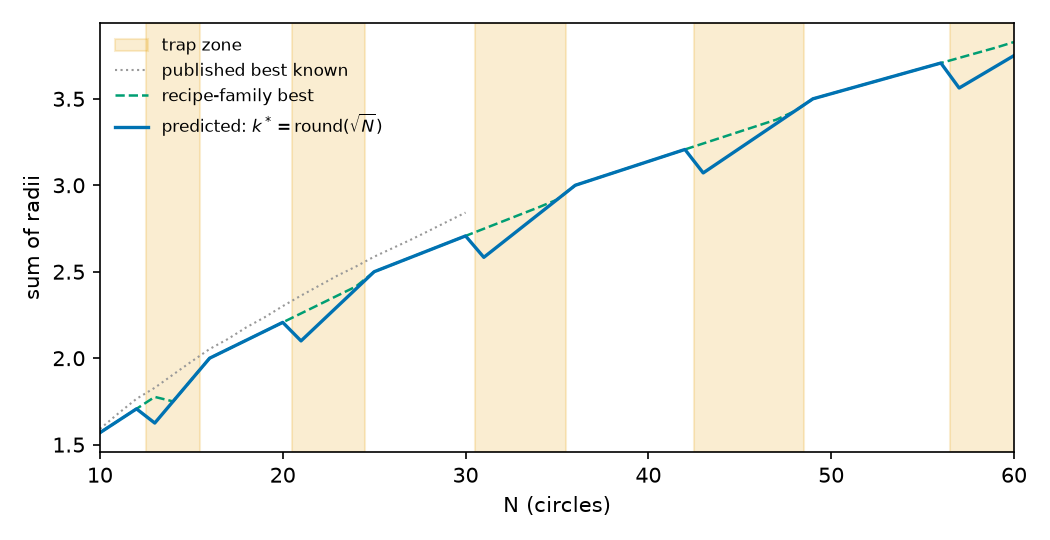
\includegraphics[width=0.78\linewidth]{fig1_trapzones.png}
\caption{\emph{Predicted versus optimal value, $N = 10\ldots60$.} (i) the rule's prediction; (ii) the
best value in the recipe family; (iii, dotted) published best-known values \citep{friedman_packing}, terminating at
$N = 30$ because the bound table stops there. Shaded bands are the trap zones, the last being
$[57,63]$ clipped by \texttt{sweep(10,60)}. Worst-in-zone penalties 8.51\%, 7.03\%, 6.01\%, 5.25\%, 4.66\%; these are
family-internal arithmetic and exact at every $N$, while the published-bound comparison (curve iii)
is checkable only up to $N = 30$, where the bound table stops. The gap
closes to zero at $N = 35$ and $N = 48$ but \textbf{not} at $N = 24$, where 0.59\% remains --- curve (ii)
sits strictly above (i) across $[21,24]$.}
\label{fig:trapzones}
\end{figure}

Branch label and penalty are not coextensive: 4 of the 22 trap-branch $N$ in range cost nothing, so
``trap'' names the branch, not a guaranteed loss. Where the penalty is zero, truncation is
separable from convergence only by structure; \S3.3 uses $N = 35$ as that control.

Every closed-form value is recomputed over the constructed coordinates by an independent linear
program that knows nothing about the recipe; the script aborts on disagreement. 83
configurations, both branches, every $k$ in $2\ldots7$, drift below $10^{-9}$.

Our bound table (\texttt{n\_sweep\_forecast.json}, transcribed from \citet{friedman_packing}) covers $N = 10\ldots30$ only, and its $N = 26$ entry, 2.63598,
\emph{is} ShinkaEvolve's figure truncated, so the LLM-driven systems are the record on this problem. What survives is that the recipe family is never competitive with that
record: deficit 0.02--0.26 across $N = 10\ldots30$, and 0.0946 at $N = 26$
($2.63598 - 2.5414214 = 0.0945586$). Above $N = 30$ there is no bound table, so both the deficit claim and the LP
gate's ``never exceeds a published bound'' abort are unchecked there, covering three of five trap
zones and four of our seven square cells.

\subsection{The recipe family: prior-arm and ledger evidence (from \S2.2)}

The finding that 94 of 95 valid proposals in prior arms were grid-plus-filler is retained only as
motivation, since those arms are not reported here; the self-contained version is the ledger
observation (\texttt{corrections\_ledger.md}, item 30) that across the 155 weak-tier rows collected before arm M only two exceeded the
family best, both by $\sim$$10^{-7}$ --- below the $10^{-6}$ bar, so neither counts as leaving the family under \S5's convention (arm M's 57 rows are scored separately in \S3.4 and were not swept
for this claim).

\subsection{The order rule is a definition, not a fitted law (from \S2.3)}

Given some $k \times k$ grid from this family, ``the nearest
square lattice'' yields $\mathrm{round}(\sqrt{N})$ by construction; $\arg\min_k |k^2 - N|$ switches at
$N = k^2 + k + \tfrac{1}{2}$, $\mathrm{round}(\sqrt{N})$ at $k^2 + k + \tfrac{1}{4}$, so on the integers the two coincide
--- two formalizations of ``nearest'' agreeing signals that no substantive hypothesis
is being selected. Scoring four candidate orders against the three fitting anchors gave
\texttt{nearest} 3/3, \texttt{floor} 2/3, \texttt{argmax} 2/3, \texttt{ceil} 1/3; under a null where each candidate matches
each anchor with probability $\tfrac{1}{2}$, some candidate among four goes 3/3 about 40\% of the time, so
this is a weakly identified discrete selection, not a zero-parameter law.

\section{Relocated from \S3 and \S4: per-arm tables and disclosures}

\subsection{The mode ceiling: structural check and scope conditions (from \S3.2)}

Post-hoc structural check, not preregistered, run after the square arm closed
(\texttt{diagnostics\_kmatch.py}): the grid order backed out of each sample's dominant radius
($k = \mathrm{round}(1/2r)$) equals $k^*(N)$. All 50 of 50 on-prediction samples are $k^*$-structured --- the
value match is not an accounting coincidence --- and 64 of 69 valid samples overall (93\%) sit on
the $k^*$ grid, so most value misses are $k^*$-grid variants (perturbed radii or filler counts), not
different constructions.

Three cells ($N = 17$, 35, 37), all non-discriminating, carry four valid samples each, where a 3/4
mode is thin evidence on its own; the well-populated cells of the held-out probe (\S3.8) are the
stronger test of the same rule. Two scope conditions: this is the bare weak-tier arm --- pooled
over the four discriminating square cells (full ledger), the two higher tiers and the rectangle,
the on-prediction rate is 46\% ($47/102 = 41/57 + 1/30 + 0/4 + 5/11$; the three non-discriminating
square cells, 9/12, are excluded because prediction equals the family argmax there), because \S5's
higher tiers are almost never on-prediction --- and ``modal'' is a property of the observed
sampling regime, not of a pinned decoding configuration (\S8).

\subsection{Forecast versus outcome, and arm F bookkeeping (from \S3.3 and \S4.2)}

\begin{table}[!ht]
\centering
\caption{Forecast versus outcome, both containers.}
\label{tab:forecast}
\small
\begin{tabular}{@{}lcccccc@{}}
\toprule
Cell & Branch & Predicted & Rival argmax & Valid / sampled & On-pred / valid & Rival \\
\midrule
$N{=}13$ (sq) & truncate & 1.6250000 & 1.7761424 & 4/5 $\cdot$ \textbf{18/20} & 3/4 $\cdot$ \textbf{10/18} & 0 \\
$N{=}17$ (sq) & extend & 2.0517767 & $\dagger$ & 4/5 & 3/4 & $\dagger$ \\
$N{=}21$ (sq) & truncate & 2.1000000 & 2.2588835 & 7/10 $\cdot$ \textbf{15/20} & 4/7 $\cdot$ \textbf{12/15} & 2 \\
$N{=}31$ (sq) & truncate & 2.5833333 & 2.7485281 & 5/5 $\cdot$ \textbf{17/20} & 5/5 $\cdot$ \textbf{13/17} & 0 \\
$N{=}35$ (sq) & truncate & 2.9166667 & $\dagger$ & 4/5 & 3/4 & $\dagger$ \\
$N{=}37$ (sq) & extend & 3.0345178 & $\dagger$ & 4/5 & 3/4 & $\dagger$ \\
$N{=}43$ (sq) & truncate & 3.0714286 & 3.2416246 & 7/10 & 6/7 & 0 \\
$N{=}19$, $a{=}3$ & truncate & 3.1666667 & 3.5749194 & 4/8 & 2/4 & 0 \\
$N{=}25$, $a{=}2$ & truncate & 3.1250000 & 3.4832492 & 7/8 & 3/7 & 0 \\
\bottomrule
\end{tabular}

\vspace{0.5ex}
\begin{minipage}{0.95\linewidth}
\footnotesize
Plain entries are the original 45-invocation bare arm (\S3.3's corpus); \textbf{bold} the same cells
over the full 85-row bare ledger after \S6 added 40 rows. $\dagger$ marks non-discriminating cells
(prediction equals family argmax), excluded from rival denominators. Square discriminating
cells: 18/23 and 2/23 on the original corpus; 41/57 and 2/57 on the full ledger. Rectangle:
5/11 and 0/11. Sources: \texttt{arm\_f\_repro.py} over \texttt{arm\_f\_candidates\_v2.jsonl}, \texttt{arm\_g\_rect.py} over
\texttt{arm\_g\_candidates.jsonl}.
\end{minipage}
\end{table}

The original-corpus figures cover the \textbf{original 45-invocation bare arm only} (ids $\le 5$ at
$N = 13/31$, $\le 10$ at $N = 21$, all rows at $N = 17/35/37/43$), the corpus that existed when \S3
was written. \S6 later added 40 bare rows at $N = 13/21/31$ under the same arm label; over the full
shipped ledger the same four cells give 41/57 on-prediction and 2/57 rival. Both are reported.

Five invocations were rejected by the runtime's 20-subagent concurrency cap
\emph{before reaching a model}. We excluded them under a rule that was not preregistered, so the arm
is reported both ways --- $35/45 = 77.8\%$, or $35/50 = 70.0\%$ had the rejections been scored as model
failures --- and the five records appear in the ledger in no form (\S9). The arm
also contains three parse failures, and one $N = 37$ proposer derived
$r = (\sqrt{2}-1)/12$ correctly in prose, then transcribed 0.03571429.

\subsection{Arm M in full (from \S3.4)}

Two gaps remained after the square arm: (i) $V(k, m)$'s filler branch
was empirically supported only at $m \in \{0, 1\}$ --- the converge cells $N = 17$ and 37 both have
$m = 1$ --- and (ii) the $k = 8$ trap zone appeared in Figure 1 but was never sampled. Arm M closes
both gaps and was registered before sampling (\texttt{arm\_m\_preregistration.txt}, commit
\texttt{e528c6b}; prompt hashes in \texttt{arm\_m\_prompts.json}): $n = 15$ bare weak-tier
invocations at each of $N = 20$ ($k^* = 4$, $m = 4$, predicted $V(4,4) = 2.2071068$), $N = 30$
($k^* = 5$, $m = 5$, $V(5,5) = 2.7071068$), $N = 41$ ($k^* = 6$, $m = 5$, $V(6,5) = 3.1725890$) and
$N = 57$ ($k^* = 8$, trap, $T(8,57) = 3.5625000$, rival $V(7,8) = 3.7366935$), with an explicit
tie-stated falsifier for each half.

The registered predictions P-M1--P-M3 are disconfirmed: not one of the three converge cells has
$V(k^*, m)$ as its modal output. The model does not extend a $k^*$-grid with fillers; it moves
\emph{up} to the $(k^*{+}1)$ grid and truncates or exactly fills it --- modal outputs
$2.0 = T(5,20)$ (12 of 15 valid; $N = 20$ is the $5 \times 4$ rectangle exactly), $2.5 = T(6,30)$
(11 of 14; $6 \times 5$ exactly) and $2.9285714 = T(7,41)$ (6 of 7; $7 \times 6$ minus one). Exactly one
sample in 36 valid converge-cell rows emitted the registered construction --- a textbook $V(4,4)$,
all four fillers at $(\sqrt{2}-1)/8$. Per the registered falsifier wording, \textbf{$V(k, m)$ is
restricted to the $m \le 1$ support previously observed}, and the branch rule's extend arm is
disconfirmed at $m \ge 4$; the intermediate ``places some fillers'' outcome named in the
registration did not occur (filler count 0 in 35 of 36 valid converge rows). The emergent
regularity is arithmetic, not geometric: where $N$ factors as $a \times b$ with $a$, $b$ near
$\sqrt{N}$ the model emits that exact rectangle of uniform circles ($20 = 5 \times 4$,
$30 = 6 \times 5$), which is further evidence for \S8's arithmetic-tractability alternative ---
rectangle factorization is mentally computable where filler tangency is not.

Validity by cell: 15/15, 14/15 (one parse failure --- fraction literals), 7/12 and 10/15 at
$10^{-6}$. Three $N = 41$ invocations died in the runtime before reaching a model and are excluded
under the rejection rule registered for this arm in \texttt{arm\_m\_preregistration.txt} ---
registered precisely because the analogous arm F exclusion was not (\S9) --- and counted here: the
cell is $n = 12$ sampled of 15 launched. Raw rows verbatim in \texttt{arm\_m\_collect.jsonl}; scoring
in \texttt{arm\_m\_analysis.py}, conventions identical to arm F.

\textbf{Table M --- Arm M, forecast versus outcome (all four registered cells).}

\begin{center}
\begin{small}
\setlength{\tabcolsep}{3.5pt}
\begin{tabular}{@{}ccp{0.09\linewidth}p{0.16\linewidth}p{0.20\linewidth}ccp{0.16\linewidth}@{}}
\toprule
$N$ & $k^*$ & Branch & Registered prediction & Modal valid output & Freq & Valid / sampled & Verdict \\
\midrule
20 & 4 & extend, $m = 4$ & $V(4,4) = 2.2071068$ & $T(5,20) = 2.0000000$ ($5 \times 4$ exact) & 12/15 & 15/15 & P-M1 \textbf{disconfirmed} \\
30 & 5 & extend, $m = 5$ & $V(5,5) = 2.7071068$ & $T(6,30) = 2.5000000$ ($6 \times 5$ exact) & 11/14 & 14/15 & P-M2 \textbf{disconfirmed} \\
41 & 6 & extend, $m = 5$ & $V(6,5) = 3.1725890$ & $T(7,41) = 2.9285714$ ($7 \times 6 - 1$) & 6/7 & 7/12 & P-M3 \textbf{disconfirmed} \\
57 & 8 & truncate & $T(8,57) = 3.5625000$, rival count 0 & $T(8,57) = 3.5625000$ & 6/10 & 10/15 & P-M4 confirmed; rival 0/10 \\
\bottomrule
\end{tabular}
\end{small}
\end{center}

Exactly one $V(k^*, m)$ construction appears in 36 valid converge-cell rows; filler count is 0
in 35 of 36. Three converge-cell rows leave the recipe family \emph{upward} --- two at $N = 20$ (staggered rows of four at $r = 1/9$, sum 2.2222222, against the family best $V(4,4) = 2.2071068$) and one at $N = 30$ ($r = 1/11$, sum 2.7272727, against $V(5,5) = 2.7071068$; valid at $10^{-6}$, not at $10^{-9}$) --- hexagonal layouts the family does not contain, found by a post-hoc sweep (not preregistered) run after a fourth-round check; they are not the modal output at either cell and do not bear on the discriminating-cell claims. Regenerates from \texttt{arm\_m\_collect.jsonl} via \texttt{arm\_m\_analysis.py}.

\subsection{Arms MU and CH in full (from \S3.5)}

Two questions were still open after arm M. Does the unconditioned anchoring result say anything
about calls that carry a parent program --- the regime evolutionary loops actually run in --- and
does the \S8 arithmetic-tractability alternative survive a direct probe? Arms MU and CH were
registered together before sampling (\texttt{arm\_mu\_preregistration.txt}, commit \texttt{2b7d202};
prompt hashes in \texttt{arm\_mu\_prompts.json}), with numeric decision thresholds, a power analysis
(0.83 at the registered effect size), tie-against conventions, and falsifier F-MU1.

\textbf{Arm MU} issues one-parent mutation calls: the bare prompt plus an existing packing and the
instruction to modify it so the sum of radii increases. Three parents per cell
($N = 13$, 21, 31; $n = 15$ per condition-cell, 135 invocations): \emph{A\_anchor}, the model's own
unconditioned anchor $T(k^*, N)$; \emph{B\_rival}, the provably better in-family rival $V(k^*{-}1, m)$;
and \emph{C\_offfamily}, a diagonal-chain packing scoring $\approx$ 0.59--0.62, far below either.
Every valid B\_rival sample keeps or refines the rival construction, and every one inherits the
rival's grid order. The template does not reassert itself when a better in-family parent is
present. A\_anchor makes the same point from the other side: even with the model's \emph{own} anchor
as parent and an explicit increase-the-sum instruction, only 7 of 28 valid samples (25\%,
CI $[0.13, 0.43]$) stay on the anchor. Per the registered falsifier wording: the unconditioned-call
anchoring result does not transfer to parent-conditioned calls, the loop-relevance framing is
disconfirmed for the one-parent regime, and this paper's claims are scoped to unconditioned calls
throughout. The one condition where the template does reassert itself is the one the registration
predicted it would: given the \emph{off-family} diagonal parent, 20 of 34 valid samples (58.8\%,
CI $[0.42, 0.74]$) abandon the parent entirely and emit a $k^*$-grid construction --- P-MU4 holds
per-cell at $N = 21$ (7/13) and $N = 31$ (12/14, every valid sample on the $k = 6$ grid), though
not at $N = 13$ (1/7). The asymmetry is the finding: a good in-family parent is followed, a bad
off-family parent is discarded for the template. The attractor is real but weak --- it captures
the trajectory only when the parent is worse than what the template supplies.

\textbf{Arm CH} hands the model the entire recipe family: the bare prompt plus every admissible
$T(k, N)$ and $V(k, m)$ value enumerated, including the family argmax, with the instruction to
use whichever scores highest or anything better ($n = 15$ per cell, 45 invocations). The \S8
tractability alternative says the model truncates at $k^*$ because that is the only construction
it can compute; enumerating the family removes the computation burden, so under that reading
the modal output should become the stated argmax (P-CH2). Under the template reading it stays
$T(k^*, N)$ despite the argmax being printed in the prompt (P-CH1). Read no further than the
registered scorer and the tractability alternative fails the probe. But validity is low in this
arm --- 2, 5 and 7 valid of 15 by cell --- and the failure modes reverse the picture at the
\emph{attempt} level: all 31 invalid rows attempt the stated argmax (every one carries the family's
filler radius). Of those, 30 misplace the fillers --- typically at the container corners, where
radius $(\sqrt{2}-1)/(2k)$ overlaps the adjacent grid circle; the correct construction places them
at the grid interstices --- and 1 emits radical literals the registered scorer cannot evaluate.
Counting attempts rather than valid outputs, the model \emph{chooses} the argmax in a large
majority of CH invocations and simply fails to execute it; the valid-conditioned modal is
dominated by the template because the template is the only construction the model executes
reliably. This is the same asymmetry arm MU found from the other direction, and it narrows the
paper's central claim to its defensible core: the template is not what the model prefers; it is
what the model can build.

\textbf{Table MU --- Arm MU, registered thresholds versus outcome, by parent condition (pooled
over $N = 13$, 21, 31).}

\begin{center}
\begin{small}
\setlength{\tabcolsep}{3.5pt}
\begin{tabular}{@{}p{0.15\linewidth}cp{0.13\linewidth}p{0.13\linewidth}p{0.10\linewidth}p{0.08\linewidth}p{0.24\linewidth}@{}}
\toprule
Parent & Valid & Anchor-rate (CI) & Registered threshold & Keep-or-improve & $k$-inher. & Reading \\
\midrule
\emph{B\_rival} (in-family argmax) & 26 & 0/26 (0\%, $[0.00, 0.13]$) & DISSOLVES if $\le$ 20\% & 26/26 (bar $\ge$ 50\%) & 26/26 & \textbf{F-MU1 triggered} --- anchoring does not transfer to one-parent calls \\
\emph{A\_anchor} (model's own anchor) & 28 & 7/28 (25\%, $[0.13, 0.43]$) & P-MU1 predicted $\ge$ 50\% & --- & --- & not met --- even the anchor-as-parent does not hold the anchor \\
\emph{C\_offfamily} (diagonal, $\approx$0.6) & 34 & 20/34 abandon parent for $k^*$-grid (58.8\%, $[0.42, 0.74]$) & P-MU4: template reasserts & --- & --- & holds at $N = 21$, 31; not at $N = 13$ (1/7) \\
\bottomrule
\end{tabular}
\end{small}
\end{center}

\textbf{Table CH --- Arm CH, valid-conditioned verdict versus attempt-level decomposition.}

\begin{center}
\begin{small}
\setlength{\tabcolsep}{3.5pt}
\begin{tabular}{@{}ccp{0.24\linewidth}cp{0.22\linewidth}p{0.21\linewidth}@{}}
\toprule
$N$ & Stated argmax & Modal valid output & Valid & Invalid rows attempting argmax & Registered verdict \\
\midrule
13 & 1.7761424 & $T(4,13) = 1.6250000$ & 2/15 & all & P-CH1 holds \\
21 & 2.2588835 & argmax, 3/5 & 5/15 & all & P-CH2 (argmax) \\
31 & 2.7485281 & $T(6,31) \approx 2.5833$ (4/7) & 7/15 & all & P-CH1 holds (one-sample margin) \\
pooled & --- & template 2 of 3 cells & 14/45 & \textbf{31/31} (30 misplaced fillers, 1 unevaluable radicals) & choice follows score table; execution fails off-template \\
\bottomrule
\end{tabular}
\end{small}
\end{center}

Raw rows verbatim in \texttt{arm\_mu\_collect.jsonl} (180 of 180 launched invocations collected across arms MU and CH, no
runtime deaths); scoring in \texttt{arm\_mu\_analysis.py}, committed before sampling completed; frozen
output in \texttt{arm\_mu\_results.txt}. This arm brings the study corpus to 468 invocations.

\subsection{Arms GM3 and V in full (from \S3.6)}

\textbf{Table CV --- Cross-vendor verdicts, both instruments.}

\begin{center}
\begin{small}
\setlength{\tabcolsep}{3.5pt}
\begin{tabular}{@{}p{0.10\linewidth}p{0.13\linewidth}p{0.14\linewidth}p{0.20\linewidth}p{0.32\linewidth}@{}}
\toprule
Vendor & Model & Instrument & Registered test & Verdict \\
\midrule
Google & gemma-4-26b & first-party API, 7 $N$ $\times$ 20 (41/140 rows routed under amendment; dual accounting) & pooled $\ge$ 30\%; cell-level $\ge$ 5; falsifier $\ge$ 4 fails & pooled bar met (57.5\%); discriminating cells 11/43 = 26\%, \textbf{below} the bar; cell-level short (2/5, falsifier not triggered); all three misses are the \emph{rival construction} (27/43) \\
Cohere & north-mini-code & free-tier alias, 5 $N$ $\times$ 5 & V1 $\ge$ 50\% of valid on-prediction; V2 rival $\le$ 10\% & \textbf{TRANSFERS}, point-estimate (8/12 = 67\%; CI includes bar); V2 HOLDS (0/4) \\
OpenAI (open-weight) & gpt-oss-20b & free-tier alias, 5 $N$ $\times$ 5 & same & \textbf{TRANSFERS}, point-estimate (11/18 = 61\%; CI includes bar); V2 HOLDS (0/9) \\
Google & gemma-4-31b & free-tier alias, 5 $N$ $\times$ 5 & same & \textbf{DOES-NOT-TRANSFER} (0/15); V2 HOLDS (0/3) \\
10 further aliases & (NVIDIA, Liquid, Poolside, inclusionAI, others; one unattributed) & free-tier & floor: $\ge$ 10 of 25 invocations valid & BELOW-FLOOR; failure taxonomies logged, no claim in either direction \\
\bottomrule
\end{tabular}
\end{small}
\end{center}

\textbf{Arm GM3.} Arm GM3 asks whether the anchoring law is a
fact about the original lineage or about weak-tier models as a class, by re-running the
unconditioned-call protocol against a second vendor's open-weight family
(gemma-4-26b-a4b-it) through its first-party API: seven $N$ cells, twenty samples each,
registered predictions and falsifier fixed before sampling (prereg chain in \S9; the
instrument's history --- a first attempt whose 4,096-token budget was consumed entirely by the
model's deliberation channel, resolved by a registered re-run at 16,384 --- is in \S8 and
Appendix~F.1, and is itself a finding about output-budget confounds in cross-vendor comparisons).
Per cell, recomputable from \texttt{arm\_gm\_gm3\_checkpoint.jsonl} by \texttt{arm\_gm3\_analysis.py}
with no arguments:

\begin{center}
\begin{tabular}{@{}ccccccc@{}}
\toprule
$N$ & predicted (4 dp) & Gemma modal sum & mode freq & valid $n$ & on-prediction & MODE-MATCH \\
\midrule
13 & 1.6250 & 1.7761 & 7/9 & 9 & 0 & no (misses upward) \\
17 & 2.0518 & \textbf{2.0518} & 19/20 & 20 & 20 & \textbf{yes} \\
21 & 2.1000 & 2.2589 & 9/18 & 18 & 8 & no (misses upward) \\
31 & 2.5833 & 2.7485 & 11/16 & 16 & 3 & no (misses upward) \\
35 & 2.9167 & \textbf{2.9167} & 15/15 & 15 & 15 & \textbf{yes} \\
37 & 3.0345 & --- & --- & 2 & 0 & UNSCOREABLE \\
43 & 3.0714 & --- & --- & 0 & 0 & UNSCOREABLE \\
\bottomrule
\end{tabular}
\end{center}

\begin{figure}[!ht]
\centering

\includegraphics[width=\linewidth]{fig_gm3_anchoring.png}
\caption{\emph{Arm GM3 modal sums against the registered prediction.} Filled green circles match the
predicted mode (the dashed line is $V(k^*, m)$ at extend cells and $T(k^*, N)$ at truncate cells) (frequencies annotated); open red triangles miss --- every miss lands above the
prediction, on the rival argmax (the modal packings carry the rival's two-radius structure,
27/27 --- \S3.6); the two largest cells are UNSCOREABLE under the registered $<$3-valid rule.
Regenerates via \texttt{fig\_gm3\_anchoring.py} from \texttt{arm\_gm3\_report.json} (itself replayed from the
raw ledger by \texttt{arm\_gm3\_analysis.py}, no arguments).}
\label{fig:gm3anchoring}
\end{figure}

The registered metric pools all cells, and the pass rides on that: by \S3.2's own convention ---
arm F's pooled rate excludes non-discriminating cells \emph{because prediction equals the family
argmax there} --- the decomposition must be stated. 35 of the 46 on-prediction packings sit in the
two non-discriminating cells (20/20 at $N = 17$, 15/15 at $N = 35$); on the three discriminating
cells the rate is 11 of 43 (25.6\%), below the bar the pooled metric passes. \textbf{The structural
signature came in under its bar}: 20 of 46 on-prediction samples (43\%, bar: half) carry the exact
two-radius grid-plus-filler decomposition. The instrument is blind by construction at truncate
cells, whose prediction is single-radius: all 20 signatures come from $N = 17$ (20 of 20), the one
extend cell among the matches, while $N = 35$'s 15 on-prediction truncations carry no filler to
detect (0 of 15). The registered verdict stands as registered; read per eligible cell, the
construction matches wherever it can be seen.

The registered signature instrument could not see the rival structure on the miss side: it tests
radii against the \emph{predicted} order $k^*$, so it is structurally blind to $(k^*{-}1)$
constructions --- which is why the 43\% signature figure coexists with a 100\% rival-structure rate
on the miss side. Read against \S8's tractability alternative, the anchor value marks where
construction-by-mental-arithmetic lands, and a family with more arithmetic reach executes the
harder in-family construction rather than truncating --- same recipe family, other branch.

\textbf{Arm V.} Arm GM3 varied the vendor while holding the instrument close to laboratory grade ---
first-party API, pinned temperature, explicit output budget, seven cells at twenty samples.
Arm V varies vendor and serving class at once, under the same byte-identical arm-F prompts
both arms inherit (SHA-256 per $N$ restated in the registration and recomputed at call time,
aborting on mismatch; the GM-chain registration pins the identical hashes), at five cells and
five samples per (model, $N$), against free-tier aliases
across seven attributed vendors (\texttt{arm\_v\_preregistration.md}, committed before sampling; three amendments,
each committed before the sampling it governs, expanded the original three-alias design to
thirteen aliases across two serving paths --- the opencode CLI and OpenRouter chat-completions ---
and raised \texttt{max\_tokens} to 24,576 after hidden-reasoning truncation emptied three models'
replies). Serving disclosures per the companion paper's protocol: aliases on managed paths,
\texttt{sampling\_params: null} on every row, per-row upstream-provider strings logged where the path
reports them, every invocation appended live to \texttt{arm\_v\_candidates\_raw.jsonl} --- 877
invocations, failures and refusals included. Scoring is \texttt{arm\_f\_repro.py}'s
parse/validate/classify unchanged, tolerances registered in arm F before its sampling.

Registered floor: $\ge$10 of a model's 25 registered invocations valid at $10^{-6}$; below it, no
anchoring claim in either direction. Execution retried each invocation slot until content
arrived, per amendment 3's registered transport-repair and accounting rule, so the ledger
holds many more attempt rows than slots --- gemma-4-31b's 25 slots, for instance, took 190
attempt rows, 165 of them transport failures --- and the floor is evaluated on the 25 slots,
not the attempts. Ten of thirteen aliases finished BELOW-FLOOR --- including all three
originally-registered opencode aliases, whose logged failure taxonomies are
transport-dominated for one (CLI build banners, timeouts, ``Unknown model'' errors as the
free tier rotated its catalogue) and roughly half transport, half parse-failure for the
other two --- plus one alias returning all 108 of its attempts without content. Three aliases
cleared the floor, and their registered verdicts split:

\begin{center}
\footnotesize
\setlength{\tabcolsep}{3.5pt}
\begin{tabular}{@{}lcccc@{}}
\toprule
alias (vendor) & valid & V1 on-prediction & V1 verdict (bar: $\ge$50\%) & V2 rival-argmax (bar: $\le$10\%) \\
\midrule
\texttt{north-mini-code} (Cohere) & 12 & 8/12 [39--86\%] & \textbf{TRANSFERS} (point est.) & 0/4 $\rightarrow$ \textbf{HOLDS} \\
\texttt{gpt-oss-20b} (OpenAI, open-weight) & 18 & 11/18 [39--80\%] & \textbf{TRANSFERS} (point est.) & 0/9 $\rightarrow$ \textbf{HOLDS} \\
\texttt{gemma-4-31b-it} (Google) & 15 & 0/15 = 0\% & \textbf{DOES-NOT-TRANSFER} & 0/3 $\rightarrow$ \textbf{HOLDS} \\
\bottomrule
\end{tabular}
\end{center}

The registration (\texttt{arm\_v\_preregistration.md}) recorded the original family's prior for the
strong-form statistic as 0/21 over $N \in \{13, 31\}$ only --- a narrower scope than \S3.3's 2/23,
whose two rival hits both sit at $N = 21$, so the two corpora agree at 0 on the registration's own
cells; \S3.6's gemma-4-26b, under the GM-chain instrument, is the standing exception --- its
discriminating-cell mode \emph{is} the rival. And the transfer is not universal: gemma-4-31b,
clearing the same floor, lands the prediction never. Its valid packings are unanchored and low
(bests 0.88--1.85 against predictions 1.63--3.03) --- not the rival, not the template, just weaker
de-novo construction.

The gemma pair needs stating precisely, because this family now appears on both sides, and
the prompts are identical across the two arms --- what differs is parameter count, serving
path and sample budget, not the elicitation. Under the GM-chain instrument (first-party,
pinned temperature, $7 \times 20$), gemma-4-\textbf{26b} met the pooled bar at 57.5\% while its discriminating-cell rate (26\%) fell below it (the mixed-serving
accounting; first-party-only, 59.0\% --- \S8's registered deviation applies to this figure)
while emitting the \emph{rival} construction at 63\% of discriminating-cell validities; under arm
V's free-tier instrument ($5 \times 5$), gemma-4-\textbf{31b} through a rate-starved alias (Google AI
Studio upstream; 27--38 of each cell's attempts returned as shared-pool 429s before content
arrived) lands neither the prediction nor the rival --- its valid packings are weaker de-novo
constructions. The pair bounds the family's behaviour rather than contradicting itself ---
one member sits \emph{above} the template's execution reach (far enough to build the
drop-and-fill rival the original family cannot), the other lands below it --- but model
variant and instrument quality change together across the two measurements, so which
difference carries the split is not attributable from this pair; either way, no
single-model measurement would have seen the boundary.

\subsection{Arm CC in full (from \S3.7)}

The design was registered and pushed to the public remote before sampling
(\texttt{arm\_cc\_preregistration.txt}, commit \texttt{285deca}): the three trap cells
$N = 13, 21, 31$, $n = 15$ weak-tier invocations per cell, prompt equal to the bare stem with
exactly two registered line replacements --- the code-free clause becomes a program contract
(standard-library \texttt{math} only, stated in the prompt) and the output clause asks for program
source. Programs run sandboxed (\texttt{python -I}, 10-second timeout, registered AST allowlist;
the executor and its four-bin smoke test were committed with the registration), and stdout is
scored by arm-F conventions unchanged.

\begin{center}
\begin{small}
\setlength{\tabcolsep}{4pt}
\begin{tabular}{@{}ccccc@{}}
\toprule
$N$ & Valid & Modal bucket (count, margin) & Anchor-rate & Above anchor \\
\midrule
13 & 12/15 & anchor 1.6250000 (2/12, one sample) & 2/12 & 2 --- 1.6614054, and the family argmax exactly \\
21 & 13/15 & anchor 2.1000000 (9/13, margin 8) & 9/13 & 0 \\
31 & 12/15 & anchor 2.5833333 (3/12, one sample) & 3/12 & 0 \\
\bottomrule
\end{tabular}
\end{small}
\end{center}

The registered decomposition row sharpens arm CH rather than repeating it: handed the family's
values, the model chooses the argmax and cannot build it by direct emission (30 of 31 invalid,
\S3.5); allowed to delegate the arithmetic to an executed program, it reaches the same argmax once
in 37 valid outputs and never passes it. Failure taxonomy: 7 of 45 programs produce geometrically
invalid packings, 1 imports \texttt{random} against the stated contract (caught by the registered
gate), none time out. Structural $k = k^*$ in 18 of 37 valid outputs. The lost mass is greedy
radius-growth heuristics converging under the lattice.

Scope, registered before sampling: this instrument measures externally-executed
standard-library arithmetic, not library-assisted optimization --- deployed loops permit
\texttt{numpy}/\texttt{scipy}, and the antecedent study's unconstrained agents wrote
\texttt{scipy} optimizers unprompted, which is why the constraint is stated in the prompt
rather than silently enforced; the library channel remains a further arm. Under the
registration's framing map the P-CC1 branch reads: anchoring extends into the math-only code
channel at these cells, and \S2.1's ``a code channel routes around the anchor'' is weakened
from an assumption to a measured negative --- the routing exists, and for this proposer it does
not lead out of the family. Raw rows verbatim in \texttt{arm\_cc\_collect.jsonl} (45 of 45
launched invocations collected, no runtime deaths); scoring \texttt{arm\_cc\_analysis.py};
frozen report \texttt{arm\_cc\_report.json} and summary \texttt{arm\_cc\_results.txt}.

The Sonnet-tier programs of arm CCS are qualitatively different search --- simulated annealing over
hand-rolled linear-congruential generators, Halton-sequence multi-restarts, force-directed
relaxation, against the weak tier's greedy radius growth --- yet their executed math-only search
never passes the family ceiling at any cell.

Taxonomy for the follow-ups: CC2 41 valid, 3 geometry-invalid, 1 blocked import; CCS 37 valid, 7
geometry-invalid, 1 timeout (the programme's first). One protocol note, disclosed: a single CC2
invocation ($N = 13$, slot 2) used runtime tools despite the no-tools dispatch wrapper; per the
arm-M convention its verbatim final message is scored like every other row. Ledgers
\texttt{arm\_cc2\_collect.jsonl} and \texttt{arm\_ccs\_collect.jsonl} (45/45 each, no runtime deaths);
runner \texttt{arm\_cc2\_analysis.py} reuses CC's registered pipeline unmodified. These arms bring
the study corpus to 603 invocations.

\subsection{Arm CN in full (from \S3.8)}

The $m \ge 4$ branch is already disconfirmed by arm M and was not re-tested. Cells with fewer than
five valid outputs were to be reported UNDERPOWERED; ties for the mode count against the
prediction.

\begin{center}
\begin{footnotesize}
\setlength{\tabcolsep}{4pt}
\begin{tabular}{llllllll}
\toprule
$N$ & $k^*$, prediction & disc. & valid [Wilson 95\%] & on-pred. & mode (count, margin) & verdict & $k^*$-struct. \\
\midrule
50 & 7, $V(7,1) = 3.5295867$ & no & 11/15 [48--89\%] & 4 & 3.5122554 (6, $+2$) & \textbf{MISS} & 10/11 \\
58 & 8, $T(8,58) = 3.6250000$ & yes & 14/15 [70--99\%] & 12 & 3.6250000 (12, $+11$) & \textbf{HIT} & 14/14 \\
62 & 8, $T(8,62) = 3.8750000$ & yes & 13/15 [62--96\%] & 13 & 3.8750000 (13, $+13$) & \textbf{HIT} & 13/13 \\
65 & 8, $V(8,1) = 4.0258883$ & no & 13/15 [62--96\%] & 9 & 4.0258871 (9, $+7$) & \textbf{HIT} & 12/13 \\
75 & 9, $T(9,75) = 4.1666667$ & yes & 12/15 [55--93\%] & 8 & 4.1666667 (8, $+6$) & \textbf{HIT} & 8/12 \\
\bottomrule
\end{tabular}
\end{footnotesize}
\end{center}

At the largest cell, $N = 75$, the four off-mode outputs are alternative constructions (a
$5 \times 15$ grid, twice; a hexagonal layout; a 12-column layout), none of them the rival
$V(8,11)$. The invalid rows are nine overlaps, two count errors and one output of fraction literals
the registered parser does not evaluate (the CH ``radical literal'' mode). Raw rows in
\texttt{arm\_cn\_collect.jsonl} (75/75 launched, none lost); eleven $N = 65$ rows were
transcribed by reconstructing the standard $8 \times 8$ grid string from the emitted filler
triple, flagged per row (\texttt{reconstructed: true}) and disclosed in \texttt{arm\_cn\_results.txt}; the reconstruction is character-identical for these standard grids, but a reader who discards those rows leaves $N = 65$ with three valid samples, below the five-row floor, and P-CN1 at 3 hits of 4 evaluable cells --- the three discriminating cells, which carry the contamination argument, are untouched. The arm brings the study corpus to 678
invocations.

\subsection{Rectangle transfer: all eleven valid proposals (from \S4.1)}

We characterize all eleven here. On-prediction: two
at $N = 19$/$a = 3$ (3.1666666667 and 3.16666673, the latter agreeing to six decimals not seven) and
three at $N = 25$/$a = 2$ (3.125 exactly). Off-prediction at $N = 25$/$a = 2$: two samples emitted a
uniform $5 \times 5$ grid at $r = 0.1$ summing to 2.5000000 --- the \emph{square} rule with no aspect correction,
$k = \mathrm{round}(\sqrt{25}) = 5$ --- plus one at 3.0 and one at 3.151875, the latter above the 3.125 prediction from outside the family and below the rival. At $N = 19$/$a = 3$, \textbf{two} further samples
exceeded the prediction from outside the family, 3.45 and 3.5, both below the rival.

\section{Relocated from \S5 and \S6: tier-ladder and elicitation detail}

\subsection{Three attractor families at one cell (from \S5)}

\begin{figure}[!ht]
\centering
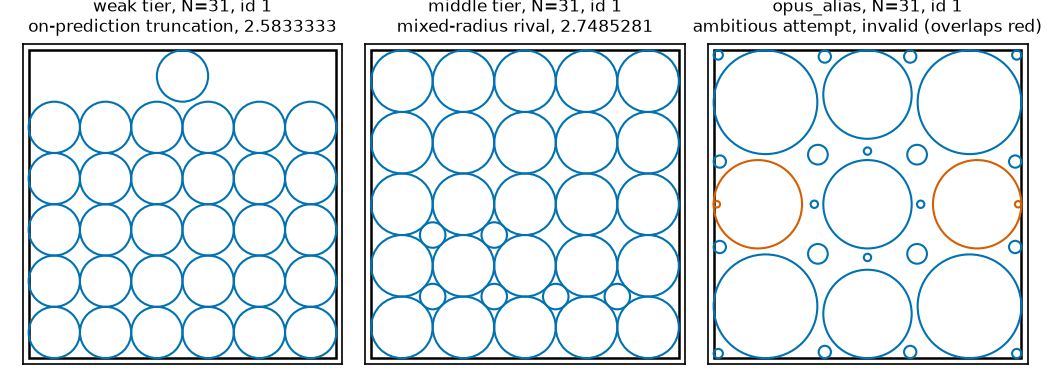
\includegraphics[width=\linewidth]{fig2_packings.png}
\caption{\emph{Three attractor families at a single cell, $N = 31$.} One representative packing
per tier, ledger sample id in each panel title (weak tier \texttt{bare} id 1, on-prediction truncation
2.5833333; middle tier \texttt{sonnet\_bare} id 1, mixed-radius rival 2.7485281; \texttt{opus\_alias} id 1,
invalid, with only the offending circles highlighted). Source: \texttt{arm\_f\_candidates\_v2.jsonl} via
\texttt{fig\_scripts.py}, deterministic (the exemplar rows' geometry is byte-identical in v1; v2 differs
only in provenance metadata).}
\label{fig:packings}
\end{figure}

\subsection{The $N = 31$ scoring defect in full (from \S5)}

One Sonnet sample at $N = 31$ emitted 27 circles at $r = 1/12$ with 4 corner circles at $r = 1/8$,
summing to 2.7499999991 --- above 2.7485281, the best the family reaches at that $N$. Recomputed
from its stored coordinates, the construction is tangency-tight: minimum pairwise and wall slack
both exactly zero at tolerance zero, the exactly-tangent contacts involving the binary-exact
$r = 1/8$ corner circles while the $r = 1/12$ circles carry small positive slack. It is the only
sample in the swept corpus (the 155 weak-tier rows before arm M, \S2.2, plus the higher tiers) to leave the recipe family upward; arm M's converge cells, scored separately, hold three more (\S3.4).

That sample also exposes a scoring defect. At $N = 31$ the family rival (2.7485281) and this
out-of-family value (2.75) differ by $1.47\times10^{-3}$, \emph{inside} the registered $2\times10^{-3}$ window, so the
value classifier counted the escape as a hit on the construction it exceeded. The window was
chosen for the anchor comparison, where the nearest competing value is $\sim$0.15 away, and reused
where it does not fit. Classified by structure instead, Sonnet's rival count at $N = 31$ is 2/10
and pooled 5/30. Every categorical claim in this paper about ``reached the
rival'' or ``left the family'' is made at structure level or at $10^{-6}$, never at $2\times10^{-3}$.

\subsection{The \texttt{opus\_alias} tolerance diagnostic (from \S5)}

Failures are geometric rather than numerical --- edge strips at $r = 0.03$ placed 0.138 from an
$r = 1/6$ grid circle needing 0.197 --- and twice the arm padded to count with zero-radius circles.
A post-hoc diagnostic (not preregistered; labeled as such in the repository) finds no tolerance
artifact behind the 13\%: 24 of 26 invalid samples overlap grossly (median maximum overlap
$3.3\times10^{-2}$; radius-shrink repair costs a median 15\% of sum-of-radii), while tolerance-scale
near-misses ($< 2.5\times10^{-5}$) fall instead in 5 of 7 geometry-scored weak-tier failures --- the
exact-tangency grids, not the ambitious constructions.

\subsection{The ambition diagnostic (from \S5)}

A post-hoc diagnostic (disclosed; \texttt{diagnostics\_ambition.py}, all samples with emitted
geometry, invalid included) gives median distinct radii per sample 1 $\rightarrow$ 2 $\rightarrow$ 3
(means 1.33 $\rightarrow$ 2.40 $\rightarrow$ 3.37) and median off-lattice center fraction 0.08
$\rightarrow$ 0.43 $\rightarrow$ 0.95 across the three tiers --- monotone on both operationalizations.

\subsection{Running corpus arithmetic (from \S6.1)}

The scaled arm ran 100 new invocations, bringing both arms to 20 per cell at
$N \in \{13, 21, 31\}$ and the corpus to 215 logged square invocations (85 bare = 45 original + 40
new; 70 trace = 10 pilot + 60 trace\_v2; 30 sonnet; 30 \texttt{opus\_alias}), plus 16 rectangle
invocations, 231 total before the extension arms. The 20 pre-existing bare rows named in \S6.1 are
$N = 13$ ids 1--5, $N = 21$ ids 1--10 and $N = 31$ ids 1--5.

Arm M (\S3.4) added 57 sampled weak-tier invocations (60 launched), bringing the study corpus to
288; arms MU and CH (\S3.5) added 180 more (180 launched, none lost); the code-channel arms CC, CC2
and CCS (\S3.7) added 135 more (135 launched, none lost), bringing the unconditioned-and-elicitation
corpus to 603; and the held-out-$N$ probe CN (\S3.8) 75 more, to 678. The cross-vendor chain is
scored under its own registrations and adds 420 GM-chain invocations (\S3.6, \S8) and 877 arm-V
attempt rows over 325 registered invocation slots (\S3.6).

\subsection{The paired trace grid (from \S6.2)}

\begin{table}[!ht]
\centering
\caption{Paired trace grid (scaled arm only).}
\label{tab:tracegrid}
\begin{tabular}{@{}llcccc@{}}
\toprule
$N$ & Arm & $n$ & Valid (parse / geom. fail) & On-pred / valid & Rival \\
\midrule
13 & bare & 20 & 18 (0 / 2) & 10 (56\%) & 0 \\
13 & trace\_v2 & 20 & 18 (0 / 2) & 16 (89\%) & 0 \\
21 & bare & 20 & 15 (1 / 4) & 12 (80\%) & 2 \\
21 & trace\_v2 & 20 & 18 (0 / 2) & 16 (89\%) & 0 \\
31 & bare & 20 & 17 (2 / 1) & 13 (76\%) & 0 \\
31 & trace\_v2 & 20 & 17 (0 / 3) & 14 (82\%) & 1 \\
\textbf{pooled} & bare & 60 & 50 (3 / 7) & 35 (70\%) & 2 \\
\textbf{pooled} & trace\_v2 & 60 & 53 (0 / 7) & 46 (87\%) & 1 \\
\bottomrule
\end{tabular}
\end{table}

\begin{figure}[!ht]
\centering
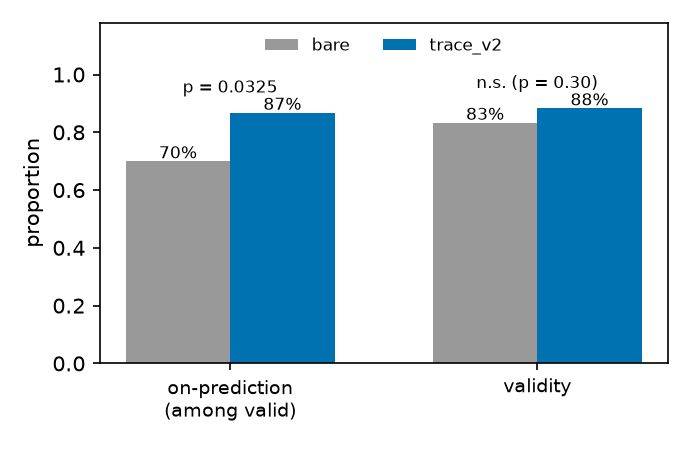
\includegraphics[width=\linewidth]{fig3_armT.png}
\caption{\emph{Bare versus \texttt{trace\_v2}, pooled over cells.} The annotated $p = 0.0325$ is uncorrected and fails the Holm threshold (\S6.4); per-cell values are in the text. Caption caveat: the bars pool the
bare arm's two collection waves, which \S6.4 shows drift materially, so the pooled bare bar is a
mixture; the same-wave comparison in \S6.4 is the wave-controlled picture.}
\label{fig:armT}
\end{figure}

\subsection{Limits of P-T3, in full (from \S6.4)}

\emph{No registered alpha.} P-T3 registered direction only; the $p$-value is a post-hoc addition.

\emph{Multiplicity.} Of four registered predictions, three are reported with $p$-values. Holm sets the
first threshold at $0.05/3 = 0.0167$; $p = 0.0325$ fails it, as it fails Bonferroni at any $m \ge 2$ and
Benjamini--Hochberg FDR at $q = 0.05$. Two-sided Fisher is $p = 0.0537$. P-T3 is nominally significant
uncorrected and is not under family-wise error control.

\emph{Concentration in one cell.} Per-cell tests give $p = 0.030$, 0.41, 0.50
(Table~\ref{tab:tracegrid}); the pooled 17-point gap is a 33-point gap at $N = 13$ averaged with 9-
and 6-point gaps elsewhere, driven by a \emph{low bare rate at $N = 13$} ($10/18 = 56\%$) rather than
a high trace rate --- the trace rate there (89\%) equals that at $N = 21$. Dropping $N = 13$, the
comparison is 30/35 vs 25/32, $p = 0.31$.

\emph{Wave confound.} The bare arm mixes two collection waves; trace\_v2 is one. Splitting bare on the
registered id boundary, with no intervention applied to either half, on-prediction is: $N = 13$, 3/4
old wave vs 7/14 new; $N = 21$, 4/7 vs 8/8; $N = 31$, 5/5 vs 8/12 --- the control arm's own
between-wave drift is comparable to the effect attributed to the manipulation. (An earlier
draft printed 2/4 vs 10/11 at $N = 21$ and a 25/37 pooled figure --- arithmetically impossible
against \S6.1's id boundary; corrected here from the ledger.) Restricting to one
wave, new-wave bare is 23/34 (68\%) against trace\_v2's 46/53 (87\%), but \textbf{this stratified
comparison is post hoc, not preregistered, no confirmatory weight} --- a diagnosis, not a rescue:
wave is a confound \emph{in the registered analysis}, which cannot separate it from the manipulation.
The design fix, interleaved collection in one session, was not run.

\subsection{The twelve exclusions of the registered faithfulness scorer (from \S6.5)}

Nine of the registered scorer's 12 exclusions are regex
coverage gaps, not claims without numeric content: \texttt{DIMS\_RE} matched only the
literal \texttt{NxN} form and \texttt{ROWSCOLS\_RE} required rows before columns, so these fell through despite
carrying explicit checkable dimensions --- ``Regular 3 by 4 grid with one additional circle in row
4''; ``3 complete rows of 4 circles and 1 centered circle in the top row''; ``rectangular grid 4-4-4-1
with uniform radius 1/8''; ``Four-row grid with 4 circles in the first row and 3 in each of the
remaining''; ``Rectangular grid arrangement with 5 columns and 4 rows, plus one additional circle on
top edge''; ``Square grid 5 columns 4 rows with 1 additional circle at top''; ``Rectangular grid six
columns by six rows radius one-twelfth with five circles removed''; ``Regular 5-column by 6-row grid
plus one additional circle in the right margin''; ``Rectangular grid packing with five columns and
six rows plus one additional circle''. Three further exclusions --- ``Uniform horizontal strips with
tight row spacing'', ``Regular rectangular grid packing with corner circle'', ``Equal-radius
rectangular grid with 4 rows stacked vertically'' --- are closer to genuinely unscoreable.

\subsection{Design and bundling disclosure, exact diffs (from \S6.1)}

The pilot's trace prompt had drifted from the bare template beyond the method line --- it omitted
the \texttt{[0,1]x[0,1]} tokens and reworded the output-format line --- so the pilot's intervention
was method-line-plus-rewording, bundled.

The scaled prompt, \texttt{trace\_v2}, is itself a \textbf{bundled prompt-format-and-trace-request}
intervention, though a near-minimal diff: one inserted \texttt{METHOD:} line, plus \texttt{"After
the METHOD line, "} prepended to the output line and \texttt{"no other text"} changed to
\texttt{"no other text after the list"}. That second change is not cosmetic --- \S6.2 shows it
doing measurable work --- so the measured effect is
\emph{method-line-plus-output-line-rewording}, not the method line alone: a weaker version of the
confound for which the pilot was discarded, held to the same standard. The Fisher exact test comes
from the hypergeometric tail in \texttt{arm\_t\_analysis.py}, checked against a reference.

\subsection{The registered falsifier, both readings, in full (from \S6.3)}

The code evaluated direction as \texttt{t\_rate >= b\_rate}, strict \texttt{<}, under which the
falsifier fires at 0 of 3 cells. That convention appears nowhere in the preregistration, was chosen
at analysis time, and read the same tie favorably twice --- as ``direction held'' for P-T1 and as
``not a falsifier cell'' here.

We name the failure mode \textbf{operationalization drift between preregistration text and analysis
code}: registered prose leaves boundary behavior --- ties, inclusive versus exclusive bounds,
rounding --- implicit, and the scorer must choose after the data exist; the preregistration
literature (\S7) discusses what is locked, not this tie-handling layer. Remedies, free before
sampling and impossible afterward: register the comparison as executable code, or state the tie
convention in the registration text. \texttt{arm\_t\_analysis.py} now prints both readings and names
the registered tie-inclusive one authoritative.

Per-cell one-sided Fisher on on-prediction (pooled bars in Figure~\ref{fig:armT}): $N = 13$
$p = 0.030$; $N = 21$ $p = 0.41$; $N = 31$ $p = 0.50$. Pooled $p = 0.0325$; Holm threshold over the
registered family ($m = 3$ tested with $p$-values) is 0.0167. The pilot (10 invocations at
$N = 21$, 10/10 valid, 9/10 on-prediction) is reported separately and never summed into any total.
Regenerated by \texttt{arm\_t\_analysis.py} over \texttt{arm\_f\_candidates\_v2.jsonl}.

\subsection{Faithfulness: rubric, mismatches and the original scorer (from \S6.5)}

The rubric (\texttt{p7\_faithfulness\_rubric.md}) fixed checkable assertions in any surface form,
plus match rules including a base-grid convention for ``grid plus additions'' claims and a
truncation convention for ``with k removed'' claims.

The two mismatches share a form: row 11 claims ``alternating rows of 4 and 3 circles'' over
observed row sizes 4,3,3,3, row 33 claims ``5 rows alternating between 5 and 4 circles'' over
observed 5,4,4,4,4 --- both \emph{mis-descriptions of alternation}, a repeating pattern named and
built for the first period only. The original scorer's three mismatches were three different claim
forms, not one; the filler-adds-rows mechanism the original scorer described was real, and the
rubric's base-grid convention handles it, so all three score MATCH under hand adjudication. Both
failures are a model describing a pattern it started and did not finish.

On scope: the original 93\% conditioned on completions that produced a correct packing --- the
wrong conditioning, since a method line attached to an overlapping layout is where description and
artifact are likeliest to diverge. Faithfulness is informative precisely on off-template outputs,
such as the pilot's triangular-hexagonal 6+5+4+3+2+1 sample, described exactly while summing to
1.75; the non-claim guard applies in full, and ``$5 \times 5$ grid'' matching a $5 \times 5$ grid is
closer to a self-consistency check than to the causal question the chain-of-thought literature
asks.

\section{Relocated from \S8 and \S9: instrument history and full provenance}

\subsection{The cross-vendor chain, instrument by instrument (from \S8)}

All tiers in the main study come from one provider; \S3.6 is the arm that moves the pooled-level
claim across vendors. The instrument's history matters as much as its verdict and is recorded
here. Arm GM (gemini-2.5-flash-lite, prereg commit \texttt{37b3adb}) stalled on first-party quota at
55 of 140 and was completed through a routed serving path under a registered amendment
(\texttt{arm\_gm\_amendment1\_openrouter.md}, provider logged per row --- every resumed row reports
Google as the upstream). Its registered verdict is UNDERPOWERED in both accountings: 20
valid packings of 140, three scoreable cells against the five the primary requires, pooled
on-prediction 15\% against the 30\% bar, falsifier not triggered
(\texttt{arm\_gm\_analysis\_v2.py}, \texttt{arm\_gm\_v2\_report.json}). Two descriptives, claimed as nothing
more: the one mid-size scoreable cell matches the predicted mode exactly (2.1000 at $N = 21$,
3/6), and off-prediction valid sums land far \emph{below} the prediction (0.48--1.55) --- the
opposite direction from GM3's misses, which land on the family rival (\S3.6), consistent
with \S5's point that the regularity is
tier-bound rather than universal. Arm GM2 (gemma-4-26b-a4b-it, prereg
\texttt{3019aab}) completed 140/140 invocations with 0 of 140 parseable --- and the two
candidate readings (format inability versus budget truncation) were separated by GM3 as
registered: the vendor API returns deliberation as a separate thought channel, GM2's
4,096-token budget died entirely inside that channel, and at 16,384 tokens the same model
parses at 123/140 (\texttt{parsed} flag in \texttt{arm\_gm3\_candidates.jsonl}). A cross-vendor null under a fixed output budget is not evidence about the
model until the budget's interaction with the vendor's response structure is itself checked.
One mechanical deviation on GM3 is on record (amendment registered before resumption): the
final 41 of 140 cells were collected through a routed third-party serving path after the
first-party quota stalled, provider logged per row, both accountings computed --- the
deviation moves the pooled rate from 59.0\% (first-party only) to 57.5\% (mixed) and changes
no verdict. Scope after \S3.6: the anchoring law is cross-vendor at the pooled level; its
full cell-level mode structure remains confirmed only within the original family. Arm V
(\S3.6) extends the chain under the zero-shot protocol: registered before sampling with three
pre-sampling amendments, 877 invocations across thirteen free-tier aliases, ten below the
registered floor with their failure taxonomies logged, and the three floor-clearing vendors
splitting TRANSFERS/TRANSFERS/DOES-NOT-TRANSFER (\texttt{arm\_v\_score.py}, no arguments, from the
live ledger; frozen output \texttt{arm\_v\_score\_final.txt}).

\subsection{Provenance limits and the confirmatory base, in full (from \S8 and \S9)}

\textbf{Sampling parameters unpinned.} The runtime does not expose pinned decoding parameters, so
every effect is a distributional claim over the observed sampling regime, and \S3.2's mode-ceiling
result inherits that scope. This is the subject of the companion paper.

\textbf{\texttt{opus\_alias} provenance.} The label denotes the serving alias addressed, not an
identified model version. Without pinned weights we cannot separate a model-tier effect from a
serving-path effect, and the supporting anomalies live only in the runtime transcript.

\textbf{One prompt, one phrasing.} Every arm conditions on a single hash-locked prompt and no
paraphrase variant was sampled, so the anchor is established as a property of the (model, prompt
string) pair; locking buys reproducibility, not robustness to rewording, and prompt-format
sensitivity of the size reported by \citet{sclar2024formatspread} is untested here. Relatedly, the
cross-vendor concentration differences in \S3.6 are measured but not explained; alignment-induced
diversity loss \citep{kirk2024rlhf} predicts vendor-dependent concentration and is a candidate
account we did not test.

\textbf{Confirmatory base for the branch rule, updated by arm M.} floor and round disagree exactly
on $N \in [k^2-k+1, k^2-1]$, so every discriminating cell is a trap cell by construction. The
truncate arm now has five confirmed $k$ in the square (4, 5, 6, 7, 8 --- the last added by arm M's
$N = 57$ cell, \S3.4) plus two rectangle cells; the extend arm is confirmed only at $m \le 1$ and
\textbf{disconfirmed at $m \ge 4$} (\S3.4), which is the sharper scope the abstract now carries. The
empirical-$k$ back-out has been run twice as disclosed post-hoc diagnostics:
\texttt{diagnostics\_kmatch.py} (\S3.2 --- 50/50 on-prediction samples $k^*$-structured, 64/69 valid
overall) and arm M's per-cell $k_{\mathrm{emp}}$ distributions (\S3.4 --- the converge cells sit on
$k^*{+}1$, which is how the filler-branch failure was diagnosed).

\textbf{The decisive experiment, as originally named (from \S8).} The one-parent mutation arm was
specified as: same cells, prompt = bare template plus one parent packing plus its score plus
``propose a modification that increases the sum of radii'', under three parent conditions (the
on-prediction truncated grid, the higher-value family rival, an off-family parent), measuring
whether the branch rule still predicts and whether the model inherits the parent's $k$. It has
since been run as arm MU (\S3.5). The separating experiment for the tractability alternative was
specified as: hand the model the recipe family explicitly, state $V(k, m)$ and the admissible $k$,
and ask it to \emph{choose} $k$; if it picks the argmax, the tractability reading stands. It has
since been run as arm CH (\S3.5), and the more ambitious tier's observed failure mode --- 24
overlaps and 2 nonpositive radii out of 26 \texttt{opus\_alias} failures --- is what that reading
predicts.

\subsection{Provenance in full (from \S9)}

\begin{itemize}
\item \textbf{Registration.} Prompts were hashed with SHA-256 and the hashes recorded before sampling,
  with the predicted values they were to be tested against: \texttt{arm\_f\_repro.py} (header, P1--P5,
  square arm), \texttt{arm\_s\_preregistration.txt}, \texttt{arm\_o\_preregistration.txt},
  \texttt{arm\_t\_preregistration.txt} (prereg hash \texttt{ab7900a8\ldots}), \texttt{arm\_m\_preregistration.txt} with
  \texttt{arm\_m\_prompts.json} (committed \texttt{e528c6b} before sampling), and
  \texttt{arm\_mu\_preregistration.txt} with \texttt{arm\_mu\_prompts.json} (committed \texttt{2b7d202} before
  sampling; decision thresholds, power analysis, tie conventions and falsifier F-MU1 all
  registered), and the cross-vendor chain \texttt{arm\_gm\_preregistration.txt} (commit \texttt{37b3adb}),
  \texttt{arm\_gm2\_preregistration.txt} (\texttt{3019aab}), \texttt{arm\_gm3\_preregistration.txt} (\texttt{c0b5b97}) with
  its serving-path deviation registered in \texttt{arm\_gm3\_amendment1\_openrouter.md} (\texttt{67cc4a1})
  before the affected cells were sampled, and \texttt{arm\_v\_preregistration.md} (commit \texttt{5444f10},
  ancestry-checked by its runners before any sampling) with its three amendments, each
  committed before the sampling it governs. Arm CC's registration
  (\texttt{arm\_cc\_preregistration.txt} with frozen prompts, executor and smoke test) was
  committed and pushed to the public remote at \texttt{285deca} before its first invocation;
  arms CC2 and CCS were registered together (\texttt{arm\_cc2\_preregistration.txt}, commit
  \texttt{4d7b7c5}, pushed before sampling) after CC's results were known, with that
  motivation disclosed in the registration itself. Arm CN (\texttt{arm\_cn\_preregistration.txt},
  commit \texttt{69a1642}, pushed before sampling) was registered after the rest of the manuscript was
  complete, in response to a pre-submission check; its motivation is post-hoc with respect to the paper's results and is
  disclosed in the registration, and its predictions were fixed before its first invocation.
  The rectangle transfer was registered before
  collection and never refitted. On multiplicity: this study now spans many registered arms, and no
  correction across arms is applied --- each arm's predictions were registered with its own
  bars and falsifiers before its sampling, every arm is reported regardless of outcome
  (three GM-chain instruments failed or stalled before one succeeded, and \S3.4's falsifier
  fired), and no arm was selected for inclusion on its result. The protection against
  garden-of-forking-paths here is registration and exhaustive reporting, not a family-wise
  error rate; a reader who wants one can count arms from this section.
\item \textbf{Four limits on that claim.} (i) The digests cover the task prompt only; the subagent
  inherits instruction files outside it, so what is locked is a \emph{fragment} of the conditioning
  context, a replicator cannot reconstruct those files, and we cannot establish they were
  identical across the arm-F and arm-T windows --- the boundary \S6.4 identifies as a confound.
  (ii) \texttt{arm\_f\_prompts.json} covers $N = 13$, 17, 31, 35 and 37; the $N = 21$ bare hash is registered
  in \texttt{arm\_t\_preregistration.txt}; the \textbf{$N = 43$ bare hash appears in no preregistration and no
  prompts file}, existing only in the ledger --- it recomputes exactly from the bare template, but
  recomputation after the fact is not registration. (iii) \textbf{No hash was ever registered for the
  pilot prompt}, whose drift the preregistration describes only in prose; the ten pilot rows
  carry \texttt{prompt\_sha256: null} in the corrected ledger with an explanatory note. (iv) The
  rectangle ledger (\texttt{arm\_g\_candidates.jsonl}) carries no prompt hashes, no run dates and no
  proposer fields at all.
\item \textbf{Ledger metadata correction.} Three internal-check findings established that the shipped ledger's
  provenance fields contradicted the paper: trace rows carried the \emph{bare} prompt hash for their
  cell, \texttt{run\_date} was uniformly \texttt{2026-07-30} on all 215 rows, and the Sonnet and \texttt{opus\_alias}
  rows were stamped with the Haiku alias and dated id. All three are corrected in
  \texttt{arm\_f\_candidates\_v2.jsonl}; the correction is metadata only --- every scored quantity, geometry,
  raw output, arm label and sample id is byte-identical to v1, verified field by field, each
  corrected field carrying a sibling \texttt{*\_v1} field. \texttt{arm\_f\_candidates.jsonl} is unmodified
  (sha256 \texttt{02ecabcd\ldots}); v2 is \texttt{9f845f78\ldots}. Correction rules, sources, wave-boundary arithmetic
  and caveats --- including that \texttt{run\_date} has day granularity only --- are in
  \textbf{\texttt{ledger\_v2\_corrections.md}}. Analysis scripts read v2.
\item \textbf{Excluded and unreleased records.} The five concurrency-cap rejections appear in the ledger
  in no form, no \texttt{excluded\_reason} field exists, and the exclusion rule was not preregistered;
  both rates are reported in \S3.3. The \texttt{opus\_alias} latency and token-count anomalies (\S5) come
  from the runtime session transcript; no latency or token field exists in any released artifact.
\item \textbf{Analysis artifacts.} Raw outputs are stored verbatim (\texttt{arm\_f\_raw.json},
  \texttt{arm\_f\_candidates.jsonl}, \texttt{arm\_f\_candidates\_v2.jsonl}, \texttt{arm\_g\_candidates.jsonl},
  \texttt{arm\_m\_collect.jsonl} scored by \texttt{arm\_m\_analysis.py}, \texttt{arm\_mu\_collect.jsonl} scored by
  \texttt{arm\_mu\_analysis.py} with frozen output \texttt{arm\_mu\_results.txt}, and the GM3 ledger
  \texttt{arm\_gm\_gm3\_checkpoint.jsonl} --- every row's raw API response verbatim, serving path and
  provider tagged per row --- scored by \texttt{arm\_gm3\_analysis.py} into \texttt{arm\_gm3\_report.json}
  with both serving-path accountings) and scoring is deterministic and local. Value claims are gated on an independent LP oracle rather than on the
  closed form being tested: \texttt{n\_sweep\_forecast.py} with \texttt{verify\_against\_lp} checks 83
  configurations to within $10^{-9}$, and the same oracle produced \S4.2's negative result. The
  faithfulness rubric (\texttt{p7\_faithfulness\_rubric.md}) was frozen by git commit \texttt{e181d2a}
  (2026-08-01 03:56:56) before any rescoring, and all 60 blind labels with justifications are in
  \texttt{p7\_blind\_labels.json}. \texttt{arm\_t\_analysis.py}, \texttt{n\_sweep\_forecast.json}, \texttt{rect\_forecast.json},
  \texttt{p11\_mode\_baseline.json} and \texttt{STATE.md} are included; every table regenerates from raw outputs
  by a command documented in \texttt{HOW\_TO\_RUN.md}.
\item \textbf{Use of AI systems.} Claude models wrote the collection harnesses, the scoring,
  analysis and verification scripts, and drafted the manuscript prose; the human author
  directed the programme, set the research questions, approved each preregistration before
  sampling, made the final inclusion, stopping and submission decisions, and is solely
  responsible for the content. The claim a reader can check is the ordering, not the
  authorship: each preregistration commit is a git ancestor of the sampling it governs.
  Because the authoring models share a family with arms under study (\S5), what a reader is
  asked to trust is the released artifact --- the scripts, raw ledgers, LP oracle and frozen
  outputs --- not the author.
\item \textbf{Internal checks.} Before submission the manuscript passed an internal adversarial
  check: language models of other families (\texttt{deepseek-v4-pro}, \texttt{deepseek-v4-flash},
  Gemini), under written protocols, independently recomputed the paper's statistics from the
  released ledger; thirty-two claims were corrected as a result, itemized in the supplementary
  \texttt{corrections\_ledger.md}. This is quality assurance, not peer review, and carries no
  external authority.
\item \textbf{Stopping rule.} The manuscript closed after implementing the internal-check
  findings; no further data-dependent analysis was performed. Arms CC, CC2 and CCS (\S3.7) and CN (\S3.8)
  were each registered, run and scored once under their own preregistrations after that
  close; each analysis script was committed before its sampling and not modified after. Analyses named but
  not run --- the one-parent mutation arm, the recipe-family choice probe, the empirical-$k$
  back-out, faithfulness split by on- versus off-prediction, a library-enabled code probe
  (\texttt{numpy}/\texttt{scipy}; the math-only code channel has since run as arm CC), interleaved
  re-collection of the arm-T pair, and P5 at $n = 20$ --- are recorded in \S6.5 and \S8 as future work,
  so that the reported statistics remain the ones the preregistrations governed.
\end{itemize}


\end{document}
